\documentclass[12pt]{article}

%==================== PACKAGES ====================
\usepackage[margin=1in]{geometry}
\usepackage{amsmath,amssymb,amsthm}
\usepackage{enumitem}
\usepackage{bm}
\usepackage{hyperref}
\usepackage{fancyhdr}
\usepackage{xcolor}
\usepackage{tabularx}
\usepackage{array}
\usepackage{booktabs}
\usepackage{tikz}
\usepackage{pgfplots}
\pgfplotsset{compat=1.17}
\usepackage[most]{tcolorbox}
\tcbuselibrary{theorems,skins,breakable}
\usepackage{graphicx}
\usepackage{multicol}
\usepackage{draftwatermark}

%==================================================
% COURSE METADATA (EDIT THESE FOR EACH MODULE)
%==================================================
\newcommand{\CourseCode}{HE2002}
\newcommand{\CourseName}{Macroeconomics II}
\newcommand{\DocType}{Revision Notes}
\newcommand{\AcademicYear}{Academic Year 2025--2026}

%==================================================
% TCOLORBOX THEOREM STYLES
%==================================================

% ---------- DEFINITION: dark green, title in darker band ----------
\newtcbtheorem[number within=section]{definition}{Definition}%
{enhanced,
breakable,
colback=green!5!white,
colframe=green!40!black,
colbacktitle=green!50!black,
coltitle=white,
fonttitle=\bfseries,
title filled,
boxed title style={
size=small,
top=2pt, bottom=2pt,
left=6pt, right=6pt,
arc=1pt, outer arc=1pt
},
boxrule=0.9pt,
arc=1pt,
left=8pt, right=8pt, top=10pt, bottom=8pt,
before skip=12pt, after skip=12pt
}{def}

% ---------- THEOREM: blue, title in darker band ----------
\newtcbtheorem[number within=section]{theorem}{Theorem}%
{enhanced,
breakable,
colback=blue!3!white,
colframe=blue!40!black,
colbacktitle=blue!55!black,
coltitle=white,
fonttitle=\bfseries,
title filled,
boxed title style={
size=small,
top=2pt, bottom=2pt,
left=6pt, right=6pt,
arc=1pt, outer arc=1pt
},
boxrule=0.9pt,
arc=1pt,
left=8pt, right=8pt, top=10pt, bottom=8pt,
before skip=12pt, after skip=12pt
}{thm}

\tcolorboxenvironment{identity}{
enhanced,
breakable,
colback=green!5!white,
colframe=green!60!black,
fonttitle=\bfseries,
boxrule=1pt,
arc=3pt,
left=8pt, right=8pt, top=8pt, bottom=8pt,
before skip=12pt, after skip=12pt
}

\tcolorboxenvironment{principle}{
enhanced,
breakable,
colback=red!5!white,
colframe=red!60!black,
fonttitle=\bfseries,
boxrule=1pt,
arc=3pt,
left=8pt, right=8pt, top=8pt, bottom=8pt,
before skip=12pt, after skip=12pt
}

%==================================================
% CUSTOM TCOLORBOX ENVIRONMENTS (WITH NAMES)
%==================================================

\newtcolorbox{keyformula}[1][]{
enhanced,
breakable,
colback=blue!5!white,
colframe=blue!75!black,
title=Key Formula,
fonttitle=\bfseries,
boxrule=0.9pt,
arc=2pt,
left=8pt, right=8pt, top=8pt, bottom=8pt,
#1
}

\newtcolorbox{examplebox}[1][]{
enhanced,
breakable,
colback=brown!5!white,
colframe=brown!75!black,
title=Worked Example,
fonttitle=\bfseries,
boxrule=0.9pt,
arc=2pt,
left=8pt, right=8pt, top=8pt, bottom=8pt,
#1
}

\newtcolorbox{commonmistake}[1][]{
enhanced,
breakable,
colback=red!5!white,
colframe=red!75!black,
title=Common Mistake,
fonttitle=\bfseries,
boxrule=0.9pt,
arc=2pt,
left=8pt, right=8pt, top=8pt, bottom=8pt,
#1
}

\newtcolorbox{policynote}[1][]{
enhanced,
breakable,
colback=yellow!10!white,
colframe=orange!75!black,
title=Policy Application,
fonttitle=\bfseries,
boxrule=0.9pt,
arc=2pt,
left=8pt, right=8pt, top=8pt, bottom=8pt,
#1
}

\newtcolorbox{examtip}[1][]{
enhanced,
breakable,
colback=purple!5!white,
colframe=purple!75!black,
title=Exam Focus,
fonttitle=\bfseries,
boxrule=0.9pt,
arc=2pt,
left=8pt, right=8pt, top=8pt, bottom=8pt,
#1
}

%==================================================
% TITLE / HEADER / FOOTER / WATERMARK
%==================================================

\title{%
\vspace{-0.5cm}
{\Large\bfseries \CourseCode\ \CourseName{} -- \DocType}
}

\author{Quantitative Research Society @ NTU}
\date{\AcademicYear}

\pagestyle{fancy}
\fancyhf{}
\fancyhead[L]{\CourseCode\ \CourseName{} -- \DocType}
\fancyhead[R]{\href{https://qrsntu.org}{QRS@NTU}}
\fancyfoot[C]{\thepage}
\renewcommand{\headrulewidth}{0.4pt}
\renewcommand{\footrulewidth}{0pt}
\setlength{\headheight}{14.5pt}

% Watermark
\SetWatermarkText{QRS@NTU --- qrsntu.org}
\SetWatermarkScale{1}
\SetWatermarkLightness{0.99}

%------------- HEADER & FOOTER (for page 2 onward) -------------
\fancypagestyle{main}{
\fancyhf{}
\fancyhead[L]{\CourseCode\ \CourseName{} -- \DocType}
\fancyhead[R]{\href{https://qrsntu.org}{QRS@NTU}}
\fancyfoot[C]{\thepage}
\renewcommand{\headrulewidth}{0.4pt}
\renewcommand{\footrulewidth}{0pt}
}

%------------- SIMPLE FOOTER (page 1 only) -------------
\fancypagestyle{plainfirst}{
\fancyhf{}
\renewcommand{\headrulewidth}{0pt}
\renewcommand{\footrulewidth}{0pt}
\fancyfoot[C]{\scriptsize\textcolor{gray}{\textit{For academic reference only.
This document is provided for educational purposes and does not constitute an
official question paper, answer key, or any formally authorised academic
material. Its content is not guaranteed to be complete or accurate.}}}
}

%------------- HYPERREF METADATA -------------
\hypersetup{
colorlinks=true,
linkcolor=blue,
filecolor=magenta,
urlcolor=cyan,
pdftitle={\CourseCode\ \CourseName{} -- \DocType},
pdfauthor={Quantitative Research Society, NTU},
pdfsubject={\CourseName},
pdfkeywords={macroeconomics, QRS@NTU, revision notes}
}

%==================================================
% DOCUMENT
%==================================================
\begin{document}
\maketitle
\thispagestyle{plainfirst}

%==================================================
% FILE: HE2002_RevisionNotes(2).tex
% REPLACE: abstract
%==================================================
\begin{abstract}
\noindent
Integrated revision notes for \CourseCode\ \CourseName. The document keeps the early short-run block (goods market, financial markets, IS--LM, and extended IS--LM) as background architecture, then concentrates revision density on Lectures 5--11: the labour market, inflation dynamics, the medium-run IS--LM--PC framework, growth, and selected challenge topics. The notes are organised around models, recurring derivations, diagrams, and policy logic rather than slide order, so that links between short-run stabilisation, natural-rate concepts, medium-run adjustment, and long-run growth remain explicit.
\end{abstract}

\vspace{0.5cm}
\newpage
\tableofcontents
\newpage

\newgeometry{left=0.7in,right=0.7in,top=1in,bottom=1in}
\fontsize{10.5pt}{11.5pt}\selectfont
\pagestyle{main}

%==================================================
% FILE: HE2002_RevisionNotes(2).tex
% REPLACE: section* Course Overview & Topic Map
%==================================================
\section*{Course Overview \& Topic Map}
\addcontentsline{toc}{section}{Course Overview \& Topic Map}
%====================================================================

\begin{center}
\renewcommand{\arraystretch}{1.3}
\setlength{\tabcolsep}{6pt}

\begin{tabularx}{\textwidth}{
|>{\raggedright\arraybackslash}p{3.2cm}
|>{\raggedright\arraybackslash}p{1.6cm}
|>{\raggedright\arraybackslash}X
|>{\raggedright\arraybackslash}p{1.8cm}|
}
\hline
\textbf{Topic Area} & \textbf{Study Weeks} & \textbf{Key Concepts} & \textbf{ILOs} \\
\hline
Goods Market (closed economy) &
Week 1 (13 Jan) &
Goods-market equilibrium, consumption, investment, government spending, taxes, multiplier logic, and the demand side of output determination. &
1,2 \\
\hline
Financial Market &
Week 2 (20 Jan) &
Money versus bonds, money demand, nominal and real interest rates, and central-bank control of the policy rate. &
1,2 \\
\hline
IS--LM Model &
Week 3 (27 Jan) &
Joint equilibrium in goods and financial markets; IS relation; LM relation; short-run policy analysis. &
1,2,4 \\
\hline
Extended IS--LM &
Week 4 (3 Feb) &
Risk premia, credit conditions, and the role of the financial system in shifting the effective borrowing rate. &
1,2,4 \\
\hline
Labor Market &
Week 5 (10 Feb) &
Employment, unemployment, participation, wage setting, price setting, WS--PS diagram, natural rate of unemployment. &
1,2 \\
\hline
Inflation and Phillips Curve &
Week 6 (17 Feb) &
Expected inflation, expectations-augmented Phillips curve, de-anchoring and re-anchoring of expectations, accelerationist Phillips curve. &
2,4 \\
\hline
Assessment checkpoint &
Week 7 (24 Feb) &
Quiz 1 / consolidation of the short-run block and labour-market block. &
1,2 \\
\hline
Recess Week &
Recess &
Catch-up, integration of IS--LM with the labour market, and preparation for the medium-run framework. &
1,2 \\
\hline
IS--LM--PC Framework &
Week 8 (10 Mar) &
Output gap, Okun's law, inflation dynamics, medium-run convergence, natural rate of interest, fiscal consolidation, oil shocks, stagflation. &
1,2,4 \\
\hline
Facts of Growth &
Week 9 (17 Mar) &
PPP, output per person versus output per worker, convergence, Malthusian trap, production function, capital accumulation versus technology. &
3 \\
\hline
Economic Growth (I) &
Week 10 (24 Mar) &
Saving, capital accumulation, depreciation, steady state, transitional dynamics, golden-rule capital, human capital. &
3 \\
\hline
Economic Growth (II) &
Week 11 (31 Mar) &
Technological progress, effective labour, balanced growth, steady state with technology, determinants of innovation, institutions. &
3 \\
\hline
Economic Growth (III) \& Challenges &
Week 12 (7 Apr) &
Robots and unemployment, inequality, redistribution, Gini coefficient, climate change, carbon pricing. &
3,4 \\
\hline
Revision \& exam preparation &
Week 13 (14 Apr) &
Cross-model synthesis across Lectures 5--11, graph revision, and distinction between short-answer analytical content and MCQ-only qualitative content. &
1,2,3,4 \\
\hline
\end{tabularx}
\end{center}

\noindent
These notes are organised by model logic rather than slide chronology. The course naturally falls into four revision blocks:
\begin{itemize}[leftmargin=1.5em]
\item \textbf{Architecture block (Lectures 1--4):} how output and interest rates are determined in the short run.
\item \textbf{Analytical core (Lectures 5--7):} natural rates, inflation dynamics, and medium-run stabilisation.
\item \textbf{Growth block (Lectures 8--10):} what determines living standards, steady states, and sustained growth.
\item \textbf{Challenge block (Lecture 11):} automation, inequality, and climate as policy extensions of growth analysis.
\end{itemize}

\begin{examtip}[title={Exam Focus: Recommended revision order}]
Use the notes in the following sequence:
\begin{enumerate}[leftmargin=1.5em]
\item \textbf{Rebuild the scaffold first:} review Chapters 1--4 only until IS, LM, real interest rates, and risk premia feel automatic.
\item \textbf{Prioritise the short-answer core:} Chapters 5--7 and 9--10 contain the densest derivations and diagrams.
\item \textbf{Then revise concept-heavy material:} Chapter 8, the later conceptual part of Chapter 10, and Chapter 11.
\item \textbf{Finish with synthesis:} use the Chapters 5--11 Summary, the formula appendix, and the notation appendix for final compression.
\end{enumerate}
If time is limited, the highest-yield path is:
\[
\text{Chapters 5--7} \;\rightarrow\; \text{Chapters 9--10} \;\rightarrow\; \text{Chapter 12 Summary} \;\rightarrow\; \text{Appendix}.
\]
\end{examtip}

\newpage

%==================================================
% FILE: HE2002_RevisionNotes(2).tex
% REPLACE: section* How to Use This Document
%==================================================
\section*{How to Use This Document}
\addcontentsline{toc}{section}{How to Use This Document}
%====================================================================

\subsection*{Structure of the Notes}

These notes are designed to sit \emph{between} your lecture slides and your tutorial problems. Each chapter is built around a repeated revision pattern:

\begin{enumerate}
\item \textbf{Core Theory} --- definitions, assumptions, equilibrium conditions, and intuition.
\item \textbf{Mathematical Framework} --- key equations, reduced forms, and the steps linking one form to another.
\item \textbf{Worked Examples} --- representative computations or comparative statics with full logic.
\item \textbf{Applications} --- policy interpretation, historical context, or real-world macro relevance.
\item \textbf{Exam Focus} --- high-yield tasks, standard scripts, and typical mistakes.
\end{enumerate}

A good three-pass workflow is:
\begin{itemize}[leftmargin=1.5em]
\item \textbf{First pass:} read chapter text together with all Definition, Theorem, and Key Formula boxes.
\item \textbf{Second pass:} cover the solutions and attempt the Worked Example logic on your own.
\item \textbf{Final pass:} revise the Summary chapter, Formula Reference, Notation, and Exam Focus / Common Mistake boxes only.
\end{itemize}

\subsection*{Recommended Revision Routes}

\begin{center}
\renewcommand{\arraystretch}{1.25}
\begin{tabularx}{\textwidth}{|p{2.8cm}|X|X|}
\hline
\textbf{Revision route} & \textbf{Use this when} & \textbf{Best chapter order} \\
\hline
Analytical route & You are weakest on derivations, graphs, and short-answer structure. & Chapters 3--4 \(\rightarrow\) 5 \(\rightarrow\) 6 \(\rightarrow\) 7 \(\rightarrow\) 9 \(\rightarrow\) 10 \\
\hline
Conceptual route & You mainly need to recognise definitions, distinctions, and policy logic. & Chapters 5 \(\rightarrow\) 8 \(\rightarrow\) 10 (conceptual part) \(\rightarrow\) 11 \(\rightarrow\) 12 \\
\hline
Final-week route & You already know the material once and want compression, comparison, and recall practice. & Chapter 12 Summary \(\rightarrow\) Formula Appendix \(\rightarrow\) Notation Appendix \(\rightarrow\) weak chapters only \\
\hline
\end{tabularx}
\end{center}

\subsection*{How the Summary and Appendix Should Be Used}

\begin{itemize}[leftmargin=1.5em]
\item \textbf{Chapter 12} is not a substitute for Chapters 5--11; it is the synthesis layer that turns separate lectures into one coherent map.
\item \textbf{Formula \& Key Results Reference} is for rapid recall and for checking sign logic before the exam.
\item \textbf{Notation} is there to prevent avoidable confusion, especially between $Y$ versus $Y_n$, $u$ versus $u_n$, $k$ versus $\tilde{k}$, and $r$ versus $i$.
\item \textbf{Exam \& Admin Information} is the final checklist, not the main revision source.
\end{itemize}

\subsection*{Colour and Box System}

The document uses a colour-coded system. Each box has a \textbf{name} at the top so that its purpose remains clear even when printed in black and white.

\begin{center}
\begin{tabular}{|l|l|p{7cm}|}
\hline
\textbf{Colour} & \textbf{Box Name} & \textbf{Use This For} \\
\hline
\colorbox{green!5}{Green} & \textbf{Definition} & Precise concepts, variables, and model primitives to be used consistently throughout the course. \\
\hline
\colorbox{blue!3}{Blue} & \textbf{Theorem} & Core results and formal statements that structure model logic. \\
\hline
\colorbox{blue!5}{Blue} & \textbf{Key Formula} & High-yield equations and identities to memorise or derive quickly. \\
\hline
\colorbox{brown!5}{Brown} & \textbf{Worked Example} & Representative tutorial-style problems with full logic. \\
\hline
\colorbox{red!5}{Red} & \textbf{Common Mistake} & Traps, false shortcuts, and sign errors that frequently appear in exams. \\
\hline
\colorbox{yellow!10}{Yellow} & \textbf{Policy Application} & Real-world interpretation or policy meaning of the model. \\
\hline
\colorbox{purple!5}{Purple} & \textbf{Exam Focus} & What to prioritise, how to answer, and what the examiner is likely testing. \\
\hline
\end{tabular}
\end{center}

\noindent
If you print in black and white, rely mainly on the box \textbf{title} rather than the colour.



%==================================================
% Main Notes
%==================================================

\newpage
% ==========================================================
% HE2002 Macroeconomics II — Chapter 1: The Goods Market
% Source materials: :contentReference[oaicite:0]{index=0}
% (This is a chapter file intended to be \input into the main template.)
% ==========================================================

\section{The Goods Market}

\subsection{GDP and the Composition of Demand}

\begin{definition}{GDP (expenditure approach) and demand components}{def:gdp_components}
Gross Domestic Product (GDP) is commonly measured using the expenditure approach:
\emph{total spending on domestically produced final goods and services}.
Key components are:
consumption $C$, investment $I$, government purchases $G$, exports $X$, and imports $IM$.
\end{definition}

\begin{keyformula}[title={Key Formula: Total demand for goods}]
\[
Z \equiv C + I + G + X - IM,
\qquad
NX \equiv X-IM.
\]
\end{keyformula}

\noindent
In these notes we focus on a \textbf{closed economy} (the baseline for HE2002 short-run analysis), so $X=IM=0$ and
\[
Z \equiv C + I + G.
\]
We also \textbf{ignore inventory investment} in the model; nevertheless, inventory adjustments provide a useful
economic mechanism for how output adjusts when production differs from desired spending (see below).

\subsection{Model Setup: Behavioural Equations and Policy Variables}

\begin{definition}{Disposable income and net taxes}{def:disposable_income}
Disposable income is income available to households after taxes net of transfers:
\[
Y_D \equiv Y - T,
\]
where $Y$ is income/output and $T$ denotes taxes minus government transfers (net taxes).
\end{definition}

\begin{definition}{Consumption function (baseline Keynesian specification)}{def:consumption_function}
Consumption is assumed to depend positively on disposable income:
\[
C = C(Y_D), \qquad \frac{dC}{dY_D} > 0.
\]
A standard linear specification is
\[
C = c_0 + c_1 Y_D,
\quad 0 < c_1 < 1,
\]
where $c_1$ is the propensity to consume and $c_0$ is autonomous consumption.
\end{definition}

\begin{keyformula}[title={Key Formula: Consumption written in terms of $Y$ and $T$}]
Using $Y_D=Y-T$,
\[
C = c_0 + c_1(Y-T).
\]
\end{keyformula}

\begin{definition}{Endogenous vs.\ exogenous variables}{def:endo_exo}
\textbf{Endogenous} variables are determined within the model (e.g.\ equilibrium output $Y$).
\textbf{Exogenous} variables are taken as given (e.g.\ policy instruments or parameters).
A bar (e.g.\ $\bar I$) indicates an exogenous constant.
\end{definition}

\noindent
For the baseline goods-market model:
\begin{itemize}
\item Investment is taken as exogenous: $I=\bar I$ (this assumption is later relaxed in IS--LM analysis).
\item Fiscal policy variables $G$ and $T$ are taken as exogenous choices of the government.
\item We ignore the interest-rate effect on consumption in this chapter.
\end{itemize}

\subsection{Goods-Market Equilibrium and Equilibrium Output}

\begin{keyformula}[title={Key Formula: Planned expenditure in a closed economy}]
With $I=\bar I$,
\[
Z = C + \bar I + G
  = \bigl[c_0 + \bar I + G - c_1T\bigr] + c_1Y.
\]
\end{keyformula}

\begin{theorem}{Equilibrium output in the baseline goods-market model}{equilibrium_output}
Goods-market equilibrium requires output to equal demand:
\[
Y = Z.
\]
Under the linear consumption function and $I=\bar I$, equilibrium output is
\[
Y
= \frac{1}{1-c_1}\Bigl[c_0 + \bar I + G - c_1T\Bigr],
\qquad 0<c_1<1.
\]
\end{theorem}

\noindent
\textbf{Derivation.} Start from the equilibrium condition $Y=Z$ and substitute for $Z$:
\[
Y = c_0 + c_1(Y-T) + \bar I + G
  = c_0 + c_1Y - c_1T + \bar I + G.
\]
Collect $Y$ terms on the left:
\[
(1-c_1)Y = c_0 + \bar I + G - c_1T.
\]
Divide by $(1-c_1)$ (positive since $0<c_1<1$) to obtain the stated expression.

\begin{definition}{Autonomous spending}{def:autonomous_spending}
In the baseline model, define \emph{autonomous spending} as the component of planned expenditure not
depending on output:
\[
A \equiv c_0 + \bar I + G - c_1T.
\]
Then equilibrium output can be written compactly as $Y=\dfrac{1}{1-c_1}A$.
\end{definition}

\begin{commonmistake}
Do not confuse:
\begin{itemize}
\item the \textbf{accounting identity} defining demand ($Z \equiv C+I+G$ in a closed economy), and
\item the \textbf{equilibrium condition} ($Y=Z$), which pins down equilibrium output.
\end{itemize}
The identity holds by definition; the equilibrium condition is an economic restriction that holds when the goods market clears.
\end{commonmistake}

\subsection{Adjustment Mechanism and the Keynesian Cross Intuition}

\noindent
Even though we ignore inventory investment in the model, unintended inventories provide intuition for why output
moves toward equilibrium:
\begin{itemize}
\item If $Y<Z$, desired spending exceeds production; inventories fall unexpectedly and firms raise production.
\item If $Y>Z$, production exceeds desired spending; inventories accumulate unexpectedly and firms cut production.
\end{itemize}

\noindent
Graphically, the Keynesian cross plots $Z$ against $Y$ together with the $45^\circ$ line (where $Z=Y$).
The intersection determines equilibrium output.

\begin{center}
\begin{tikzpicture}[scale=0.95]
  \draw[->] (0,0) -- (8,0) node[below] {$Y$};
  \draw[->] (0,0) -- (0,6) node[left] {$Z$};

  % 45-degree line
  \draw (0,0) -- (7.2,5.4) node[above right] {$Z=Y$};

  % Demand line Z = A + c1 Y (illustrative)
  \draw (0,1.2) -- (7.2,4.8) node[above right] {$Z = A + c_1Y$};

  % Mark an equilibrium point (illustrative)
  \draw[dashed] (4.8,0) -- (4.8,3.6);
  \draw[dashed] (0,3.6) -- (4.8,3.6);
  \fill (4.8,3.6) circle (2pt) node[above left] {$Y^\ast$};
\end{tikzpicture}
\end{center}

\subsection{Fiscal Multipliers in the Baseline Model}

\begin{keyformula}[title={Key Formula: Multipliers (holding other exogenous variables fixed)}]
From
\(
Y=\dfrac{1}{1-c_1}\bigl[c_0+\bar I+G-c_1T\bigr],
\)
\[
\frac{\partial Y}{\partial G} = \frac{1}{1-c_1},
\qquad
\frac{\partial Y}{\partial T} = -\frac{c_1}{1-c_1}.
\]
\end{keyformula}

\noindent
\textbf{Interpretation.}
Government spending enters demand one-for-one, while taxes affect demand only through consumption.
A one-unit increase in $T$ reduces disposable income by one unit, but consumption falls only by $c_1$ units.

\begin{keyformula}[title={Key Formula: Geometric-series intuition for the multiplier}]
If autonomous spending increases by $\Delta A$, then output rises in successive rounds:
\[
\Delta Y
= \Delta A + c_1\Delta A + c_1^2\Delta A + \cdots
= \frac{1}{1-c_1}\Delta A.
\]
\end{keyformula}

\begin{examplebox}[title={Worked Example (Tutorial 1, Question 1): Equilibrium GDP, disposable income, consumption}]
\textbf{Given} (billions of euros):
\[
C = 480 + 0.5Y_D,\quad I=110,\quad T=70,\quad G=250.
\]
Solve for:
\begin{enumerate}[label=(\alph*)]
\item equilibrium output $Y$,
\item disposable income $Y_D$,
\item consumption $C$.
\end{enumerate}

\textbf{Solution.}
Disposable income is
\[
Y_D = Y - T = Y - 70.
\]
Substitute into the consumption function:
\[
C = 480 + 0.5(Y-70)
  = 480 + 0.5Y - 35
  = 445 + 0.5Y.
\]
Total demand (closed economy) is
\[
Z = C + I + G
  = (445 + 0.5Y) + 110 + 250
  = 805 + 0.5Y.
\]
Equilibrium requires $Y=Z$:
\[
Y = 805 + 0.5Y
\;\Rightarrow\;
0.5Y = 805
\;\Rightarrow\;
Y = 1610.
\]
Then
\[
Y_D = Y - 70 = 1610 - 70 = 1540,
\qquad
C = 480 + 0.5\cdot 1540 = 480 + 770 = 1250.
\]
\end{examplebox}


\newpage
\subsection{Balanced Budget Multiplier}

\begin{examplebox}[title={Worked Example (Tutorial 1, Question 3): Balanced budget multiplier}]
Start from the equilibrium expression
\[
Y = \frac{1}{1-c_1}\bigl[c_0 + \bar I + G - c_1T\bigr],
\qquad 0<c_1<1.
\]
\begin{enumerate}[label=(\alph*)]
\item By how much does $Y$ increase when $G$ increases by one unit?
\item By how much does $Y$ change when $T$ increases by one unit?
\item Why are the answers to (a) and (b) different?
\item Suppose initially $G=T$ and policy changes keep the budget balanced: $\Delta G=\Delta T=1$.
What is $\Delta Y$? Are balanced-budget changes neutral?
\item How does the value of $c_1$ affect your answer to (d)?
\end{enumerate}

\textbf{Solution.}
\begin{enumerate}[label=(\alph*)]
\item Differentiate with respect to $G$:
\[
\frac{\partial Y}{\partial G} = \frac{1}{1-c_1}.
\]
So a one-unit increase in $G$ raises $Y$ by $\dfrac{1}{1-c_1}$.

\item Differentiate with respect to $T$:
\[
\frac{\partial Y}{\partial T} = -\frac{c_1}{1-c_1}.
\]
So a one-unit increase in $T$ reduces $Y$ by $\dfrac{c_1}{1-c_1}$.

\item A change in $G$ shifts demand directly (one-for-one).
A change in $T$ affects demand only through consumption via disposable income, so only the fraction $c_1$ feeds into spending.

\item With $\Delta G=\Delta T=1$,
\[
\Delta Y
= \frac{1}{1-c_1}\Delta G - \frac{c_1}{1-c_1}\Delta T
= \frac{1}{1-c_1} - \frac{c_1}{1-c_1}
= 1.
\]
Thus a balanced-budget increase in $(G,T)$ is \textbf{not} neutral: output rises by one unit.

\item The balanced-budget multiplier is
\(
\Delta Y = 1
\)
for any $0<c_1<1$.
While $\dfrac{\partial Y}{\partial G}$ and $\dfrac{\partial Y}{\partial T}$ depend on $c_1$, their balanced-budget net effect does not.
\end{enumerate}
\end{examplebox}



\newpage
\subsection{Automatic Stabilizers: Income-Dependent Taxes}

\begin{definition}{Automatic stabilizers (in the goods-market model)}{def:automatic_stabilizers}
Taxes often increase with income. If net taxes follow
\(
T=t_0+t_1Y
\)
with $0<t_1<1$, then part of any increase in income is automatically taxed away,
dampening fluctuations in disposable income, consumption, and output.
\end{definition}

\begin{examplebox}[title={Worked Example (Tutorial 1, Question 4): Income-dependent taxes and the multiplier}]
Consider:
\[
C = c_0 + c_1Y_D,\qquad
T = t_0 + t_1Y,\qquad
Y_D = Y - T,
\]
with constant $G$ and $I=\bar I$, and $0<t_1<1$.
\begin{enumerate}[label=(\alph*)]
\item Solve for equilibrium output $Y$.
\item What is the multiplier on autonomous spending? Compare $t_1=0$ vs.\ $t_1>0$.
\item Explain why this tax system acts as an automatic stabilizer.
\end{enumerate}

\textbf{Solution.}
First compute disposable income:
\[
Y_D = Y - (t_0+t_1Y) = (1-t_1)Y - t_0.
\]
Then consumption is
\[
C = c_0 + c_1Y_D
  = c_0 + c_1\bigl[(1-t_1)Y - t_0\bigr]
  = (c_0 - c_1t_0) + c_1(1-t_1)Y.
\]

\begin{enumerate}[label=(\alph*)]
\item Goods-market equilibrium $Y=C+\bar I+G$ implies
\[
Y = (c_0 - c_1t_0) + c_1(1-t_1)Y + \bar I + G.
\]
Move the $Y$ term to the left:
\[
\bigl[1-c_1(1-t_1)\bigr]Y = (c_0 - c_1t_0) + \bar I + G.
\]
Hence
\[
Y = \frac{(c_0 - c_1t_0) + \bar I + G}{1-c_1(1-t_1)}.
\]

\item The multiplier on autonomous spending (the numerator term) is
\[
\frac{1}{1-c_1(1-t_1)}.
\]
If $t_1=0$, it reduces to $\dfrac{1}{1-c_1}$.
If $t_1>0$, then $1-c_1(1-t_1) > 1-c_1$, so the multiplier is smaller:
income-dependent taxes dampen the response of $Y$ to shocks.

\item When $Y$ rises, $T$ rises automatically, reducing $Y_D$ and hence moderating the increase in $C$.
When $Y$ falls, $T$ falls automatically, cushioning $Y_D$ and $C$.
This automatic offset stabilizes output without requiring discretionary policy changes.
\end{enumerate}
\end{examplebox}

\begin{policynote}
\textbf{Policy implication (short run).}
In the baseline goods-market framework, discretionary fiscal expansions (higher $G$ or lower $T$) increase equilibrium output through the multiplier.
With income-dependent taxes, the economy becomes less sensitive to shocks: automatic stabilizers reduce the effective multiplier, dampening both booms and recessions.
\end{policynote}

\subsection{Investment Equals Saving: An Equivalent Equilibrium Condition}

\begin{definition}{Private, public, and national saving}{def:saving_definitions}
Private saving is disposable income not consumed:
\[
S \equiv Y_D - C = Y - T - C.
\]
Public saving is the government budget surplus:
\[
T-G \quad \bigl(>0\ \text{surplus},\ <0\ \text{deficit}\bigr).
\]
National saving is the sum of private and public saving: $S + (T-G)$.
\end{definition}

\begin{keyformula}[title={Key Formula: Investment equals national saving (closed economy)}]
Starting from goods-market equilibrium $Y=C+I+G$,
\[
Y - T - C = I + G - T.
\]
Since $S \equiv Y-T-C$, this becomes
\[
S = I + G - T
\quad\Longleftrightarrow\quad
I = S + (T-G).
\]
\end{keyformula}

\begin{commonmistake}
In a closed economy with a government, the correct saving--investment relation is
\[
I = S + (T-G),
\]
not $I=S$.
Forgetting the public saving term $(T-G)$ leads to incorrect conclusions about how fiscal deficits relate to investment.
\end{commonmistake}

\noindent
\textbf{Deriving the same equilibrium output via saving.}
From $C=c_0+c_1(Y-T)$, private saving is
\[
S = Y - T - C
  = Y - T - c_0 - c_1(Y-T)
  = -c_0 + (1-c_1)(Y-T).
\]
Impose the equilibrium condition $I = S + (T-G)$ with $I=\bar I$:
\[
\bar I = \bigl[-c_0 + (1-c_1)(Y-T)\bigr] + (T-G).
\]
Expand and collect $Y$ terms:
\[
\bar I = -c_0 + (1-c_1)Y - (1-c_1)T + T - G
      = -c_0 + (1-c_1)Y + c_1T - G.
\]
Move constants to the right:
\[
(1-c_1)Y = c_0 + \bar I + G - c_1T
\quad\Rightarrow\quad
Y = \frac{1}{1-c_1}\bigl[c_0+\bar I+G-c_1T\bigr],
\]
which matches Theorem~\ref{thm:equilibrium_output}.

\begin{examtip}
High-frequency exam tasks for the goods-market chapter:
\begin{itemize}
\item Write down the model primitives and classify variables as endogenous vs.\ exogenous.
\item Derive equilibrium output algebraically from $Y=Z$; simplify carefully.
\item Compute $\frac{\partial Y}{\partial G}$ and $\frac{\partial Y}{\partial T}$; explain intuitively why the tax multiplier differs.
\item Solve for $Y$ under a balanced-budget change $\Delta G=\Delta T$ and interpret the result.
\item Use the saving framework to show $I=S+(T-G)$ and derive equilibrium output as a consistency check.
\item Explain (in words) how income-dependent taxes reduce the multiplier and why this is an automatic stabilizer.
\end{itemize}
\end{examtip}




\newpage
% ==========================================================
% HE2002 Macroeconomics II — Chapter 2: Financial Markets I
% Source materials: :contentReference[oaicite:0]{index=0} 
% (This is a chapter file intended to be \input into the main template.)
% ==========================================================

\section{Financial Markets I: Money, Bonds, and Interest Rates}

\subsection{Assets: Money vs.\ Bonds (Baseline Setup)}

\begin{definition}{Money, currency, and checkable deposits}{def:money_components}
In this chapter, \textbf{money} refers to assets that can be used for transactions and pay no interest.
Two canonical forms are:
\begin{itemize}
  \item \textbf{Currency}: physical cash (notes and coins).
  \item \textbf{Checkable deposits}: funds in checking accounts used for transactions.
\end{itemize}
\end{definition}

\begin{definition}{Bonds and the nominal interest rate}{def:bonds_interest}
A \textbf{bond} is a financial asset that promises a future payment. Bonds typically pay a positive \textbf{nominal interest rate} $i$ (the opportunity cost of holding money).
Money pays no interest but provides liquidity (transaction services).
\end{definition}

\noindent
We work with a stylised asset menu: households allocate financial wealth between \textbf{money} and \textbf{bonds}.
Money provides transactions services; bonds provide interest income but are not directly usable for transactions.

\subsection{The Demand for Money}

\begin{definition}{Nominal income and transactions demand}{def:nominal_income_transactions}
Let $\$Y$ denote \textbf{nominal income} (nominal GDP), a proxy for the volume of transactions in the economy.
A higher $\$Y$ increases the desired amount of money held for transactions.
\end{definition}

\begin{definition}{Money demand function}{def:money_demand_function}
Nominal money demand is assumed to take the form
\[
M^d = \$Y \, L(i),
\]
where $L(\cdot)$ is a decreasing function of the nominal interest rate $i$:
\[
L'(i) < 0.
\]
\end{definition}

\begin{keyformula}[title={Key Formula: Comparative statics of money demand}]
Holding $\$Y$ fixed, an increase in $i$ reduces money demand:
\[
\frac{\partial M^d}{\partial i} = \$Y\,L'(i) < 0.
\]
Holding $i$ fixed, an increase in $\$Y$ increases money demand:
\[
\frac{\partial M^d}{\partial (\$Y)} = L(i) > 0.
\]
\end{keyformula}

\begin{commonmistake}
\textbf{Movement vs.\ shift of the money-demand curve.}
\begin{itemize}
  \item A change in the interest rate $i$ causes a \textbf{movement along} the money-demand curve.
  \item A change in nominal income $\$Y$ causes a \textbf{shift} of the money-demand curve (since the entire schedule $M^d(i)$ is rescaled by $\$Y$).
\end{itemize}
Changes in money supply $M^s$ do \emph{not} shift money demand; they shift the money-\emph{supply} schedule.
\end{commonmistake}

\subsection{Case I: Determining the Interest Rate (Central Bank Only)}

\begin{definition}{Money supply under direct central-bank control (Case I)}{def:money_supply_case1}
In Case I, the central bank directly sets the nominal money supply at a constant level:
\[
M^s = M,
\]
represented as a vertical schedule in the $(M,i)$ plane.
\end{definition}

\begin{theorem}{Money-market equilibrium and interest-rate determination (Case I)}{thm:money_market_eq_case1}
Money-market equilibrium requires money supply to equal money demand:
\[
M^s = M^d
\quad\Longleftrightarrow\quad
M = \$Y\,L(i).
\]
Assuming $L$ is strictly decreasing and invertible, the equilibrium interest rate is
\[
i^\ast = L^{-1}\!\left(\frac{M}{\$Y}\right).
\]
\end{theorem}

\noindent
\textbf{Comparative statics (implicit differentiation).}
From $M=\$Y L(i)$:
\begin{itemize}
  \item Holding $\$Y$ fixed, differentiate w.r.t.\ $M$:
  \[
  1 = \$Y L'(i)\,\frac{di}{dM}
  \quad\Longrightarrow\quad
  \frac{di}{dM} = \frac{1}{\$Y L'(i)} < 0.
  \]
  Thus, an increase in money supply lowers the equilibrium interest rate.
  \item Holding $M$ fixed, differentiate w.r.t.\ $\$Y$:
  \[
  0 = L(i) + \$Y L'(i)\,\frac{di}{d(\$Y)}
  \quad\Longrightarrow\quad
  \frac{di}{d(\$Y)} = -\frac{L(i)}{\$Y L'(i)} > 0.
  \]
  Thus, higher nominal income raises the equilibrium interest rate (for fixed $M$).
\end{itemize}

\subsection{Open Market Operations (Implementation Intuition)}

\begin{definition}{Open market operations}{def:omo}
\textbf{Open market operations (OMO)} are central-bank purchases or sales of bonds in the bond market to change the money supply.
\begin{itemize}
  \item \textbf{Expansionary OMO}: central bank buys bonds $\Rightarrow$ money supply increases.
  \item \textbf{Contractionary OMO}: central bank sells bonds $\Rightarrow$ money supply decreases.
\end{itemize}
\end{definition}

\noindent
A minimal balance-sheet representation (stylised) is:
\begin{center}
\begin{tabular}{|p{6.2cm}|p{6.2cm}|}
\hline
\textbf{Central Bank Assets} & \textbf{Central Bank Liabilities} \\
\hline
Bonds & Money (issued by the central bank) \\
\hline
\end{tabular}
\end{center}

\noindent
An expansionary OMO increases bond holdings on the asset side and increases money on the liability side by the same amount; the opposite holds for a contractionary OMO.

\begin{policynote}
\textbf{Interest-rate targeting.}
Instead of choosing $M$ directly, a central bank can choose a target interest rate $i^{\text{target}}$ and adjust money supply through OMO so that equilibrium $M=\$Y L(i^{\text{target}})$ holds. This is a choice of \emph{operating procedure}; the equilibrium condition is unchanged.
\end{policynote}

\subsection{Bond Prices and Yields}

\begin{definition}{One-period bond yield}{def:bond_yield_one_period}
Consider a one-period bond that pays face value $F$ in one year and has price $P_B$ today.
The nominal interest rate (yield) $i$ satisfies
\[
(1+i)P_B = F.
\]
Equivalently,
\[
i = \frac{F-P_B}{P_B}.
\]
\end{definition}

\begin{keyformula}[title={Key Formula: Price--yield inversion}]
For a one-period bond paying $F$ in one year,
\[
P_B = \frac{F}{1+i},
\qquad
i = \frac{F}{P_B}-1.
\]
Hence $P_B$ and $i$ move in opposite directions.
\end{keyformula}

\begin{theorem}{Inverse relation between bond prices and interest rates}{thm:bond_price_yield_inverse}
For $F>0$ and $i>-1$,
\[
P_B(i)=\frac{F}{1+i}
\quad\Longrightarrow\quad
\frac{dP_B}{di}=-\frac{F}{(1+i)^2}<0.
\]
Thus bond prices are strictly decreasing in interest rates.
\end{theorem}

\begin{examplebox}[title={Worked Example (Tutorial 2, Question 4): Bond pricing and yields}]
A one-year bond promises to pay $\$100$ in one year.
\begin{enumerate}[label=(\alph*)]
  \item Compute the interest rate $i$ if today's bond price is $\$75$, $\$85$, and $\$95$.
  \item State the relationship between the bond price and the interest rate.
  \item If the interest rate is $8\%$, compute the bond price today.
\end{enumerate}

\textbf{Solution.}
Let $F=100$ and $P_B$ be today's price. The yield is
\[
i=\frac{F}{P_B}-1=\frac{F-P_B}{P_B}.
\]

\begin{enumerate}[label=(\alph*)]
  \item
  \begin{itemize}
    \item If $P_B=75$:
    \[
    i=\frac{100}{75}-1=\frac{4}{3}-1=\frac{1}{3}=0.333\overline{3}
    \quad\Rightarrow\quad
    i=33.\overline{3}\%.
    \]
    \item If $P_B=85$:
    \[
    i=\frac{100}{85}-1=\frac{15}{85}=\frac{3}{17}\approx 0.1764706
    \quad\Rightarrow\quad
    i\approx 17.65\%.
    \]
    \item If $P_B=95$:
    \[
    i=\frac{100}{95}-1=\frac{5}{95}=\frac{1}{19}\approx 0.0526316
    \quad\Rightarrow\quad
    i\approx 5.26\%.
    \]
  \end{itemize}

  \item From $i(P_B)=\frac{100}{P_B}-1$, we have $\frac{di}{dP_B}=-\frac{100}{P_B^2}<0$.
  Thus \textbf{bond price and interest rate are inversely related}.

  \item If $i=0.08$, then $(1.08)P_B=100$, so
  \[
  P_B=\frac{100}{1.08}=\frac{10000}{108}=\frac{2500}{27}\approx 92.59.
  \]
\end{enumerate}
\end{examplebox}


\newpage
\subsection{The Liquidity Trap and the Zero Lower Bound}

\begin{definition}{Liquidity trap (zero lower bound)}{def:liquidity_trap}
The economy is in a \textbf{liquidity trap} when the nominal interest rate has fallen to (approximately) zero,
so conventional monetary policy cannot reduce it further:
\[
i \approx 0.
\]
At $i=0$, once transaction needs are satisfied, agents can become (approximately) indifferent between holding money and bonds,
so additional increases in money supply do not lower $i$ further.
\end{definition}

\begin{theorem}{Monetary policy ineffectiveness in a liquidity trap (case-I intuition)}{thm:liquidity_trap_ineffective}
Suppose the interest rate is constrained by $i\ge 0$ and money demand becomes perfectly elastic at $i=0$ (agents absorb additional money without requiring a lower interest rate).
Then, for sufficiently large money supply increases, the equilibrium remains at
\[
i^\ast = 0,
\]
so further expansionary open market operations do not reduce $i$.
\end{theorem}

\begin{commonmistake}
Do not conclude that an expansionary open market purchase \emph{must} lower the interest rate.
When $i$ is already at (or extremely close to) zero and the economy is in a liquidity trap,
the interest rate may not change even if money supply increases.
\end{commonmistake}

\subsection{Case II: Central Bank and Commercial Banks (Monetary Base)}

\begin{definition}{Banks, deposits, and reserves}{def:banks_reserves}
Banks are financial intermediaries with \textbf{checkable deposits} as liabilities.
They hold \textbf{reserves} (assets) to meet withdrawals and settlement needs.
Central-bank money consists of \textbf{currency} plus \textbf{bank reserves}.
\end{definition}

\begin{definition}{Monetary base and reserve ratio (no-currency assumption)}{def:monetary_base}
Let $H$ denote the \textbf{monetary base} (central-bank money).
Assume households hold no currency, so money held by the public is entirely checkable deposits.
Let $\theta\in(0,1)$ be the reserve ratio, so banks desire reserves proportional to deposits:
\[
H^d = \theta M^d.
\]
In this no-currency setup, reserves coincide with the monetary base: $H=\text{reserves}$.
\end{definition}

\begin{keyformula}[title={Key Formula: Demand for monetary base (Case II)}]
If money demand by the public is
\[
M^d = \$Y L(i),
\]
and banks demand reserves $H^d=\theta M^d$, then
\[
H^d = \theta\,\$Y\,L(i).
\]
\end{keyformula}

\begin{definition}{Supply of monetary base}{def:base_supply}
In Case II, the central bank controls the supply of monetary base:
\[
H^s = H,
\]
and equilibrium in the market for central-bank money requires $H^s=H^d$.
\end{definition}

\begin{theorem}{Interest-rate determination with banks (Case II)}{thm:money_market_eq_case2}
Equilibrium in the market for central-bank money satisfies
\[
H = \theta\,\$Y\,L(i).
\]
Assuming $L$ is strictly decreasing and invertible, the equilibrium interest rate is
\[
i^\ast = L^{-1}\!\left(\frac{H}{\theta\,\$Y}\right).
\]
An increase in $H$ lowers $i^\ast$.
\end{theorem}

\begin{definition}{Money multiplier (no-currency case)}{def:money_multiplier}
With no currency held by households and reserve ratio $\theta$, deposits (money) are proportional to the monetary base:
\[
M = \frac{1}{\theta}H.
\]
The \textbf{money multiplier} is
\[
m \equiv \frac{M}{H} = \frac{1}{\theta}.
\]
\end{definition}

\begin{commonmistake}
\textbf{Monetary base vs.\ money supply.}
In Case II, the central bank directly controls $H$ (the monetary base), not total money $M$.
Total money is linked to $H$ via the money multiplier (under the maintained assumptions).
Mixing up $H$ and $M$ leads to incorrect policy predictions.
\end{commonmistake}


\newpage
\subsection{Worked Examples: Money Demand and Money-Market Equilibrium}

\begin{examplebox}[title={Worked Example (Tutorial 2, Question 2): Money demand levels and proportional shifts}]
Suppose nominal income is $\$Y=50{,}000$ (billion dollars) and money demand is
\[
M^d = \$Y\,(0.2-0.8i),
\]
where $i$ is expressed as a decimal (e.g.\ $1\%=0.01$).
\begin{enumerate}[label=(\alph*)]
  \item Compute $M^d$ when $i=1\%$ and when $i=5\%$.
  \item State how $M^d$ varies with $\$Y$ and with $i$.
  \item If $\$Y$ falls by $20\%$, what happens (in percent) to $M^d$ when $i=1\%$? when $i=5\%$?
\end{enumerate}

\textbf{Solution.}
\begin{enumerate}[label=(\alph*)]
  \item For $i=0.01$:
  \[
  0.2-0.8i=0.2-0.8(0.01)=0.192,
  \qquad
  M^d=50{,}000\times 0.192=9{,}600.
  \]
  For $i=0.05$:
  \[
  0.2-0.8i=0.2-0.8(0.05)=0.16,
  \qquad
  M^d=50{,}000\times 0.16=8{,}000.
  \]

  \item Rewrite as $M^d=\$Y\cdot(0.2-0.8i)$.
  Holding $i$ fixed, $M^d$ is proportional to $\$Y$ (higher income $\Rightarrow$ higher transactions demand).
  Holding $\$Y$ fixed, $M^d$ decreases linearly in $i$ (higher opportunity cost $\Rightarrow$ lower money holdings).

  \item If $\$Y$ falls by $20\%$, then $\$Y' = 0.8\,\$Y$ and
  \[
  (M^d)'=\$Y'(0.2-0.8i)=0.8\,\$Y(0.2-0.8i)=0.8\,M^d.
  \]
  Therefore $M^d$ falls by exactly $20\%$ for any fixed $i$, including $1\%$ and $5\%$.
\end{enumerate}
\end{examplebox}

\begin{examplebox}[title={Worked Example (Tutorial 2, Question 3): Equilibrium interest rate and a higher target}]
Suppose money demand is
\[
M^d = \$Y\,(0.25-i),
\]
with $\$Y=40{,}000$ and money supply $M^s=\$8{,}000$. Interest rates are decimals.
\begin{enumerate}[label=(\alph*)]
  \item Find the equilibrium interest rate.
  \item If the central bank wants $i=10\%$, will there be excess money supply or excess money demand at the old $M^s$?
        What change in $M^s$ is required to reach the new equilibrium?
\end{enumerate}

\textbf{Solution.}
\begin{enumerate}[label=(\alph*)]
  \item Money-market equilibrium requires $M^d=M^s$:
  \[
  40{,}000(0.25-i)=8{,}000.
  \]
  Divide by $40{,}000$:
  \[
  0.25-i=0.2
  \quad\Rightarrow\quad
  i=0.05=5\%.
  \]

  \item At $i=0.10$, money demand is
  \[
  M^d(0.10)=40{,}000(0.25-0.10)=40{,}000(0.15)=6{,}000.
  \]
  With $M^s=8{,}000$, we have $M^s-M^d=2{,}000>0$, so there is \textbf{excess money supply}.
  To make $i=10\%$ an equilibrium, set $M^s$ equal to demand at $i=0.10$:
  \[
  M^{s,\text{new}}=6{,}000,
  \]
  i.e.\ reduce money supply by $2{,}000$ via a contractionary operation.
\end{enumerate}
\end{examplebox}

\subsection{Federal Funds Rate (Institutional Anchor)}

\begin{definition}{Federal funds market and the federal funds rate}{def:ffr}
The \textbf{federal funds market} is the market for bank reserves.
The \textbf{federal funds rate} is the interest rate determined in this market and is a primary operational indicator of U.S.\ monetary policy.
In the Case II logic, the central bank influences this rate by changing the supply of monetary base $H$.
\end{definition}

\begin{examtip}
Typical exam tasks for Financial Markets I:
\begin{itemize}
  \item Start from $M^d=\$Y L(i)$ and clearly state why $L'(i)<0$.
  \item Distinguish \textbf{movements along} vs.\ \textbf{shifts} of money demand; identify what changes $M^d$ vs.\ $M^s$.
  \item Solve equilibrium interest rates from $M^s=M^d$ (Case I) or $H=\theta \$Y L(i)$ (Case II).
  \item Use implicit differentiation to sign $di/dM$ and $di/d(\$Y)$.
  \item Compute bond yields from prices and prices from yields; state and justify the inverse relation.
  \item Liquidity trap logic: explain why increasing money supply may fail to reduce $i$ when $i$ is at (approximately) zero.
\end{itemize}
\end{examtip}


\newpage
% ==========================================================
% HE2002 Macroeconomics II — Chapter 3: IS--LM Model
% (This is a chapter file intended to be \input into the main template.)
% ==========================================================

\section{IS--LM Model}

\subsection{From goods-market equilibrium to the IS relation}

Lecture 3 extends the basic goods-market model by allowing investment to depend on both output and the interest rate.

\begin{definition}{Investment relation}{}
Investment depends positively on output (or sales) and negatively on the nominal interest rate:
\[
I = I(Y,i),
\qquad
\frac{\partial I}{\partial Y}>0,
\qquad
\frac{\partial I}{\partial i}<0.
\]
Higher output raises desired investment because firms wish to expand capacity when sales are stronger. A higher interest rate raises the cost of borrowing and reduces investment.
\end{definition}

\begin{keyformula}[title={Key Formula: Goods-market equilibrium with interest-sensitive investment}]
\[
Y = C(Y-T) + I(Y,i) + G.
\]
\end{keyformula}

\noindent
This equilibrium condition is the \textbf{IS relation}. It gives the combinations of output $Y$ and the interest rate $i$ for which the goods market is in equilibrium.

\begin{theorem}{Why the IS curve is downward sloping}{}
Holding fiscal policy and other exogenous demand shifters fixed, an increase in the interest rate reduces investment demand. Lower investment reduces total demand, so equilibrium output must fall. Therefore the IS curve is downward sloping in the $(Y,i)$ plane.
\end{theorem}

\noindent
The logic is:
\[
i\uparrow \;\Rightarrow\; I\downarrow \;\Rightarrow\; Z\downarrow \;\Rightarrow\; Y\downarrow.
\]

\subsection{Linear IS equation and algebraic form}

To obtain a closed-form expression, use the standard linear specifications
\[
C = c_0 + c_1(Y-T),
\qquad
I = b_0 + b_1Y - b_2 i,
\]
with
\[
0<c_1<1,\qquad b_1\ge 0,\qquad b_2>0,\qquad c_1+b_1<1.
\]

\begin{keyformula}[title={Key Formula: Linear IS relation}]
Substituting into goods-market equilibrium gives
\[
Y = c_0 + c_1(Y-T) + b_0 + b_1Y - b_2 i + G.
\]
Hence
\[
(1-c_1-b_1)Y = c_0 + b_0 + G - c_1T - b_2 i,
\]
so
\[
Y
=
\frac{c_0+b_0+G-c_1T-b_2 i}{1-c_1-b_1}.
\]
\end{keyformula}

\noindent
For graphing in the $(Y,i)$ plane, it is often useful to write the IS relation in inverse form:
\[
i
=
\frac{c_0+b_0+G-c_1T}{b_2}
-
\frac{1-c_1-b_1}{b_2}Y.
\]
Thus
\[
\frac{di}{dY}
=
-\frac{1-c_1-b_1}{b_2}<0,
\]
confirming the downward slope.

\begin{commonmistake}
Do not say that a change in the interest rate \emph{shifts} the IS curve. A change in $i$ causes a \textbf{movement along} a given IS curve. The IS curve shifts only when some other exogenous component of demand changes, such as $G$, $T$, consumer confidence, or autonomous investment.
\end{commonmistake}

\subsection{Shifts of the IS curve}

\begin{definition}{IS-curve shifts}{}
Any change in exogenous variables that affects demand for goods at a given interest rate shifts the IS curve.
\end{definition}

\noindent
Important cases:
\begin{itemize}[leftmargin=1.5em]
\item $G\uparrow \Rightarrow$ IS shifts right.
\item $T\uparrow \Rightarrow$ disposable income falls $\Rightarrow$ consumption falls $\Rightarrow$ IS shifts left.
\item $c_0\uparrow$ or $b_0\uparrow \Rightarrow$ IS shifts right.
\item A fall in consumer confidence or autonomous investment shifts IS left.
\end{itemize}

\begin{examtip}[title={Exam Focus: Shift versus movement on IS}]
In the IS relation:
\begin{itemize}[leftmargin=1.5em]
\item \textbf{Interest-rate change} $\Rightarrow$ movement along IS.
\item \textbf{Fiscal or confidence change} $\Rightarrow$ shift of IS.
\end{itemize}
A common MCQ trap is to describe a fall in consumer confidence as an LM shift. It is an \textbf{IS shift to the left} because it lowers desired spending.
\end{examtip}

\subsection{Financial markets and the LM relation}

Lecture 2 derived money-market equilibrium as
\[
M = \$Y\,L(i).
\]
Using $\$Y = PY$, divide through by the price level:
\[
\frac{M}{P}=Y\,L(i).
\]

\begin{definition}{Real money-market equilibrium}{}
The money market is in equilibrium when real money supply equals real money demand:
\[
\frac{M}{P}=Y\,L(i),
\qquad
L'(i)<0.
\]
Real money demand rises with income and falls with the interest rate.
\end{definition}

\noindent
In the modern presentation used in Lecture 3, the central bank does not primarily think of policy as choosing $M$. Instead, it chooses a target interest rate and adjusts money supply as needed to achieve that rate.

\begin{keyformula}[title={Key Formula: LM relation under interest-rate targeting}]
\[
i=\bar{i}.
\]
\end{keyformula}

\noindent
So the LM curve is horizontal at the policy rate chosen by the central bank.

\begin{policynote}
A monetary expansion in this lecture means a \textbf{reduction in the policy interest rate}:
\[
\bar{i}\downarrow
\quad\Longleftrightarrow\quad
M\uparrow \text{ as needed to support the lower rate.}
\]
Similarly, a monetary contraction means
\[
\bar{i}\uparrow
\quad\Longleftrightarrow\quad
M\downarrow \text{ relative to what would be needed at a lower rate.}
\]
\end{policynote}

\begin{commonmistake}
Do not confuse the \emph{money-market equilibrium condition}
\[
\frac{M}{P}=Y\,L(i)
\]
with the \emph{LM relation used in this lecture}
\[
i=\bar{i}.
\]
The first is the underlying market-clearing condition. The second reflects the central bank's operating procedure: it chooses $i$ and supplies whatever money is necessary for the money market to clear at that rate.
\end{commonmistake}

\subsection{Joint equilibrium: the IS--LM model}

\begin{theorem}{Joint equilibrium in goods and financial markets}{}
The short-run equilibrium of the economy is determined by the intersection of:
\begin{itemize}[leftmargin=1.5em]
\item the \textbf{IS curve}, which gives goods-market equilibrium, and
\item the \textbf{LM curve}, which gives financial-market equilibrium under the chosen policy rate.
\end{itemize}
At the intersection, both goods and financial markets are in equilibrium simultaneously.
\end{theorem}

\begin{center}
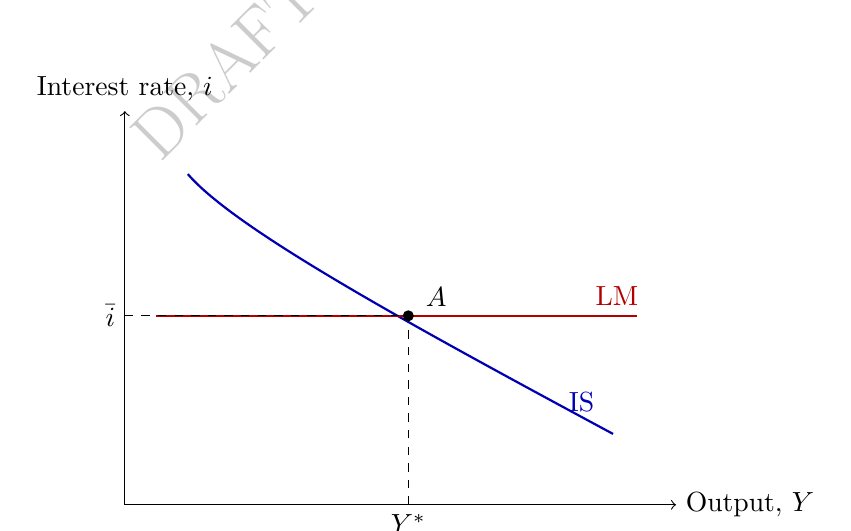
\begin{tikzpicture}[x=1cm,y=1cm]
\draw[->] (0,0) -- (7,0) node[right] {Output, $Y$};
\draw[->] (0,0) -- (0,5) node[above] {Interest rate, $i$};

% IS
\draw[thick,blue!70!black] (0.8,4.2) .. controls (1.4,3.5) and (3.6,2.3) .. (6.2,0.9);
\node[blue!70!black] at (5.8,1.3) {IS};

% LM
\draw[thick,red!70!black] (0.4,2.4) -- (6.5,2.4);
\node[red!70!black] at (6.25,2.65) {LM};

% Equilibrium
\fill (3.6,2.4) circle (2pt);
\node[above right] at (3.7,2.4) {$A$};
\draw[dashed] (3.6,0) -- (3.6,2.4);
\node[below] at (3.6,0) {$Y^\ast$};
\draw[dashed] (0,2.4) -- (3.6,2.4);
\node[left] at (0,2.4) {$\bar{i}$};
\end{tikzpicture}
\end{center}

\noindent
The graph should be read carefully:
\begin{itemize}[leftmargin=1.5em]
\item any point on IS satisfies goods-market equilibrium only;
\item any point on LM satisfies financial-market equilibrium only;
\item only their intersection satisfies both.
\end{itemize}

\subsection{Algebraic solution of the IS--LM equilibrium}

Since the LM relation is
\[
i=\bar{i},
\]
substitute directly into the IS equation.

\begin{keyformula}[title={Key Formula: Equilibrium output under interest-rate targeting}]
\[
Y^\ast
=
\frac{c_0+b_0+G-c_1T-b_2\bar{i}}{1-c_1-b_1}.
\]
\end{keyformula}

\noindent
This expression gives several immediate comparative statics:
\[
\frac{\partial Y^\ast}{\partial G}=\frac{1}{1-c_1-b_1}>0,
\qquad
\frac{\partial Y^\ast}{\partial T}=-\frac{c_1}{1-c_1-b_1}<0,
\qquad
\frac{\partial Y^\ast}{\partial \bar{i}}=-\frac{b_2}{1-c_1-b_1}<0.
\]

\noindent
Thus:
\begin{itemize}[leftmargin=1.5em]
\item higher government spending raises output;
\item higher taxes reduce output;
\item a higher policy interest rate reduces output.
\end{itemize}

\begin{examplebox}[title={Worked Example (Tutorial 3): Output, investment, and accommodating money supply}]
Consider
\[
C = c_0 + c_1(Y-T),
\qquad
I = b_0 + b_1Y - b_2 i,
\qquad
i=\bar{i}.
\]
Then:
\begin{enumerate}[leftmargin=1.5em,label=(\alph*)]
\item Goods-market equilibrium gives
\[
Y^\ast
=
\frac{c_0+b_0+G-c_1T-b_2\bar{i}}{1-c_1-b_1}.
\]
\item Equilibrium investment is
\[
I^\ast
=
b_0+b_1Y^\ast-b_2\bar{i}.
\]
\item If money demand is
\[
\frac{M}{P}=d_1Y-d_2 i,
\]
then, at the chosen interest rate $\bar{i}$, equilibrium requires
\[
\frac{M^s}{P}=d_1Y^\ast-d_2\bar{i}.
\]
So when fiscal policy raises output while the central bank keeps $i=\bar{i}$ fixed, real money supply must increase to accommodate the higher money demand.
\end{enumerate}
\end{examplebox}

\subsection{Fiscal policy in the IS--LM model}

With the interest rate held fixed by the central bank, fiscal policy works through shifts in the IS curve.

\begin{definition}{Fiscal expansion and fiscal contraction}{}
A \textbf{fiscal expansion} is an increase in $G-T$.
A \textbf{fiscal contraction} is a decrease in $G-T$.
\end{definition}

\noindent
Under interest-rate targeting:
\begin{itemize}[leftmargin=1.5em]
\item $G\uparrow$ or $T\downarrow \Rightarrow$ IS shifts right $\Rightarrow Y^\ast\uparrow$.
\item $G\downarrow$ or $T\uparrow \Rightarrow$ IS shifts left $\Rightarrow Y^\ast\downarrow$.
\item The interest rate does \emph{not} change because the central bank keeps $i=\bar{i}$ fixed.
\end{itemize}

\begin{examtip}[title={Exam Focus: Fiscal policy when LM is horizontal}]
In this version of IS--LM, fiscal expansion raises output without raising the interest rate, because the central bank accommodates the increase in money demand needed to maintain $i=\bar{i}$. So the usual crowding-out story through a higher interest rate is absent here.
\end{examtip}

\subsection{Monetary policy in the IS--LM model}

Monetary policy operates by changing the target interest rate and hence shifting the LM curve.

\begin{definition}{LM-curve shifts}{}
Since the LM relation is
\[
i=\bar{i},
\]
a change in $\bar{i}$ shifts the entire LM curve:
\begin{itemize}[leftmargin=1.5em]
\item $\bar{i}\downarrow \Rightarrow$ LM shifts down.
\item $\bar{i}\uparrow \Rightarrow$ LM shifts up.
\end{itemize}
\end{definition}

\noindent
The resulting effects are:
\begin{itemize}[leftmargin=1.5em]
\item \textbf{Monetary expansion:} $\bar{i}\downarrow \Rightarrow Y^\ast\uparrow$.
\item \textbf{Monetary contraction:} $\bar{i}\uparrow \Rightarrow Y^\ast\downarrow$.
\end{itemize}

\noindent
Graphically, a lower LM curve intersects the IS curve further to the right, so equilibrium output increases.

\begin{commonmistake}
A change in $\bar{i}$ does \textbf{not} shift the IS curve. It shifts LM. The economy then moves \emph{along} the existing IS curve to a new equilibrium.
\end{commonmistake}

\subsection{Policy mix and comparative-statics logic}

A \textbf{policy mix} is the combination of fiscal and monetary policy.

\begin{policynote}[title={Policy Application: Expansionary policy mix}]
If the economy is in recession and output is too low, policymakers can use:
\begin{itemize}[leftmargin=1.5em]
\item a fiscal expansion (IS shifts right),
\item a monetary expansion (LM shifts down),
\item or both together.
\end{itemize}
A combined fiscal and monetary expansion unambiguously raises output.
\end{policynote}

\begin{policynote}[title={Policy Application: Fiscal consolidation with monetary expansion}]
If the government wants to reduce the budget deficit without causing a recession, it may combine:
\begin{itemize}[leftmargin=1.5em]
\item \textbf{fiscal consolidation} (IS shifts left), with
\item \textbf{monetary expansion} (LM shifts down).
\end{itemize}
If the monetary expansion is large enough, output can be maintained even while the deficit is reduced.
\end{policynote}

\begin{examplebox}[title={Worked Example: Simultaneous fiscal expansion and monetary contraction}]
Suppose there is a fiscal expansion and a monetary contraction at the same time.
\begin{itemize}[leftmargin=1.5em]
\item Fiscal expansion shifts IS right.
\item Monetary contraction shifts LM up.
\end{itemize}
Then the equilibrium interest rate must rise, because the LM curve itself moves to a higher interest-rate level. However, the effect on output is \textbf{ambiguous}: the rightward IS shift raises output, while the upward LM shift lowers it. Without magnitudes, the direction of output cannot be determined with certainty.
\end{examplebox}

\subsection{How to analyse any IS--LM shock}

\begin{examtip}[title={Exam Focus: Standard 4-step method}]
For comparative-statics questions:
\begin{enumerate}[leftmargin=1.5em]
\item Identify whether the shock affects goods demand or monetary policy.
\item Decide which curve shifts: IS, LM, or both.
\item Determine the direction of the shift.
\item Read off the new equilibrium effects on output and the interest rate.
\end{enumerate}
This is the safest way to answer both diagrammatic and conceptual MCQs.
\end{examtip}

\subsection{Short-run interpretation}

The IS--LM model is the core short-run stabilisation framework:
\begin{itemize}[leftmargin=1.5em]
\item the \textbf{IS side} captures demand for goods;
\item the \textbf{LM side} captures financial-market equilibrium under the central bank's chosen interest rate;
\item the intersection determines short-run output.
\end{itemize}

\begin{theorem}{Short-run macroeconomic interpretation}{}
In the short run, output is demand-determined. Fiscal policy affects output by shifting the IS curve. Monetary policy affects output by shifting the LM curve through changes in the policy interest rate. The IS--LM model therefore provides the benchmark framework for analysing stabilisation policy before moving to medium-run inflation and labour-market adjustments in later lectures.
\end{theorem}


\newpage
% ==========================================================
% HE2002 Macroeconomics II — Chapter 4: Extended IS--LM
% (This is a chapter file intended to be \input into the main template.)
% ==========================================================

\section{Extended IS--LM}

\subsection{Why the baseline IS--LM model needs extension}

In the baseline IS--LM model, we effectively made three simplifying assumptions:
\begin{itemize}[leftmargin=1.5em]
    \item there are only two financial assets, money and bonds;
    \item there is only one relevant interest rate;
    \item all borrowing rates move one-for-one with the policy rate set by the central bank.
\end{itemize}

\noindent
Lecture 4 relaxes these assumptions. In practice:
\begin{itemize}[leftmargin=1.5em]
    \item the \textbf{central bank} controls a short-term \textbf{nominal policy rate};
    \item households and firms care about the \textbf{real cost of borrowing};
    \item actual borrowing rates differ across borrowers because of \textbf{risk premia};
    \item the health of \textbf{financial intermediaries} affects credit conditions and therefore aggregate demand.
\end{itemize}

\begin{definition}{Core idea of the extended IS--LM model}{}
The extended IS--LM model distinguishes:
\begin{itemize}[leftmargin=1.5em]
    \item the \textbf{policy rate} chosen by the central bank,
    \item the \textbf{real interest rate} relevant for spending decisions, and
    \item the \textbf{borrowing rate} actually faced by consumers and firms.
\end{itemize}
This allows financial-market disruptions to affect output even if the central bank does not change its policy rate.
\end{definition}

\subsection{Nominal versus real interest rates}

\begin{definition}{Nominal interest rate and real interest rate}{}
The \textbf{nominal interest rate} $i_t$ is the return in money terms.  
The \textbf{real interest rate} $r_t$ is the return in goods or purchasing-power terms.
\end{definition}

\noindent
Suppose one good costs $P_t$ today and the expected price level next period is $P_{t+1}^e$. If one unit of goods is converted into money today, invested at nominal rate $i_t$, and converted back into goods next period, then:
\[
1+r_t = (1+i_t)\frac{P_t}{P_{t+1}^e}.
\]

\begin{keyformula}[title={Key Formula: Exact relation between nominal and real interest rates}]
\[
1+r_t = (1+i_t)\frac{P_t}{P_{t+1}^e}.
\]
\end{keyformula}

\noindent
Define expected inflation between $t$ and $t+1$ by
\[
\pi_{t+1}^e \equiv \frac{P_{t+1}^e-P_t}{P_t}.
\]
Then
\[
P_{t+1}^e = P_t(1+\pi_{t+1}^e),
\]
so the exact relation becomes
\[
1+r_t = \frac{1+i_t}{1+\pi_{t+1}^e}.
\]

\begin{keyformula}[title={Key Formula: Fisher relation (exact and approximate)}]
\[
1+r_t = \frac{1+i_t}{1+\pi_{t+1}^e},
\qquad
r_t \approx i_t - \pi_{t+1}^e
\quad
\text{when } i_t \text{ and } \pi_{t+1}^e \text{ are not too large.}
\]
\end{keyformula}

\begin{theorem}{Comparative statics of the real interest rate}{}
Holding the nominal interest rate fixed:
\[
\frac{\partial r_t}{\partial \pi_{t+1}^e}<0.
\]
So higher expected inflation lowers the real interest rate, while lower expected inflation raises it.
\end{theorem}

\noindent
This matters because investment and other interest-sensitive spending decisions depend on the \textbf{real} borrowing cost, not the nominal rate alone.

\begin{definition}{Ex-ante and ex-post real interest rates}{}
The \textbf{ex-ante real interest rate} uses expected inflation:
\[
r_t^{\,\text{ex-ante}} \approx i_t-\pi_{t+1}^e.
\]
The \textbf{ex-post real interest rate} uses actual inflation:
\[
r_t^{\,\text{ex-post}} \approx i_t-\pi_{t+1}.
\]
\end{definition}

\begin{commonmistake}
Do not reverse the units:
\begin{itemize}[leftmargin=1.5em]
    \item the \textbf{nominal} interest rate is measured in money terms;
    \item the \textbf{real} interest rate is measured in goods or purchasing-power terms.
\end{itemize}
\end{commonmistake}

\subsection{Which interest rate enters the IS relation?}

The central bank chooses a \textbf{nominal policy rate}. However, spending decisions are driven by the \textbf{real interest rate}.

\begin{definition}{Interest rate relevant for aggregate demand}{}
The interest rate entering the IS relation is the \textbf{real interest rate}, because firms and households care about borrowing costs in terms of goods:
\[
r \approx i - \pi^e.
\]
\end{definition}

\noindent
Thus, if the central bank wants to achieve a target real interest rate $r$, it must choose the nominal interest rate $i$ taking expected inflation into account:
\[
i \approx r + \pi^e.
\]

\begin{examplebox}[title={Worked Example: Real versus nominal rate}]
Suppose the central bank wants the real interest rate to be $4\%$ and expected inflation is $2\%$. Then the required nominal interest rate is approximately
\[
i \approx r+\pi^e = 4\%+2\% = 6\%.
\]
So the central bank must set the nominal rate at about $6\%$ to obtain a real rate of $4\%$.
\end{examplebox}

\subsection{The zero lower bound and the lower bound on the real rate}

In practice, conventional monetary policy faces a lower bound on the nominal interest rate:
\[
i \ge 0.
\]

\begin{theorem}{Lower bound on the real interest rate}{}
Because
\[
r = i-\pi^e,
\]
and the nominal interest rate cannot be reduced below zero under the zero lower bound,
the lowest real interest rate the central bank can achieve is
\[
r_{\min} = -\pi^e.
\]
\end{theorem}

\noindent
This has two immediate implications:
\begin{itemize}[leftmargin=1.5em]
    \item if expected inflation is positive, the central bank may still achieve a negative real rate;
    \item if expected inflation is negative (expected deflation), the lower bound on the real rate becomes \emph{positive}, making monetary stimulus much harder.
\end{itemize}

\begin{examplebox}[title={Worked Example: Real-rate lower bound}]
\begin{enumerate}[label=(\alph*)]
    \item If expected inflation is $\pi^e=2\%$, then
    \[
    r_{\min} = -2\%.
    \]
    \item If expected inflation is $\pi^e=-2\%$ (expected deflation), then
    \[
    r_{\min} = 2\%.
    \]
\end{enumerate}
So deflation raises the lowest feasible real rate and tightens the monetary-policy constraint.
\end{examplebox}

\begin{examtip}[title={Exam Focus: Expected inflation and the real rate}]
For a \emph{given nominal interest rate}, a fall in expected inflation raises the real interest rate:
\[
r \approx i-\pi^e.
\]
Hence lower expected inflation is contractionary for interest-sensitive demand.
\end{examtip}

\subsection{Risk and risk premia}

Not all bonds are equally safe. Risky borrowers must pay a rate above the risk-free rate.

\begin{definition}{Risk premium}{}
Let $i$ denote the nominal interest rate on a riskless bond and let $x$ denote the \textbf{risk premium}. Then the risky borrowing rate is
\[
i+x.
\]
The premium $x$ compensates lenders for default risk and other forms of financial risk.
\end{definition}

\noindent
In the simple default-risk example from the lecture, let $p$ be the probability of default. If the risky bond pays nothing in default and lenders must be indifferent between risky and riskless lending, then
\[
1+i = (1-p)(1+i+x)+p\cdot 0.
\]

\begin{keyformula}[title={Key Formula: Risk premium in a simple default model}]
From
\[
1+i = (1-p)(1+i+x),
\]
we obtain
\[
x = \frac{(1+i)p}{1-p}.
\]
\end{keyformula}

\begin{theorem}{Determinants of the risk premium}{}
The risk premium increases when:
\begin{itemize}[leftmargin=1.5em]
    \item the probability of default $p$ increases;
    \item lenders become more risk averse;
    \item financial conditions deteriorate and intermediation becomes impaired.
\end{itemize}
\end{theorem}

\noindent
Thus even if the central bank keeps the policy rate unchanged, the borrowing rate faced by firms and households can rise because $x$ rises.

\begin{commonmistake}
Do not confuse:
\begin{itemize}[leftmargin=1.5em]
    \item the \textbf{policy rate}, chosen by the central bank, and
    \item the \textbf{borrowing rate}, faced by private agents.
\end{itemize}
In the extended model, these are generally \emph{not} the same.
\end{commonmistake}

\subsection{Financial intermediaries, balance sheets, and leverage}

Much real-world borrowing does not take place through direct finance alone. It goes through \textbf{financial intermediaries} such as banks, money-market funds, mortgage companies, and other non-bank institutions.

\begin{definition}{Bank balance sheet}{}
A simplified bank balance sheet satisfies
\[
\text{Assets} = \text{Liabilities} + \text{Capital}.
\]
\begin{itemize}[leftmargin=1.5em]
    \item \textbf{Liabilities}: deposits and other borrowing.
    \item \textbf{Assets}: reserves, loans, mortgages, government bonds, and other securities.
    \item \textbf{Capital}: the bank's own funds or equity cushion.
\end{itemize}
\end{definition}

\begin{center}
\renewcommand{\arraystretch}{1.25}
\begin{tabular}{|p{0.34\textwidth}|p{0.28\textwidth}|p{0.22\textwidth}|}
\hline
\textbf{Assets} & \textbf{Liabilities} & \textbf{Capital} \\
\hline
100 & 80 & 20 \\
\hline
\end{tabular}
\end{center}

\begin{definition}{Capital ratio and leverage ratio}{}
For the balance sheet above:
\[
\text{Capital ratio}=\frac{\text{Capital}}{\text{Assets}}=\frac{20}{100}=20\%,
\]
\[
\text{Leverage ratio}=\frac{\text{Assets}}{\text{Capital}}=\frac{100}{20}=5.
\]
The leverage ratio is the inverse of the capital ratio.
\end{definition}

\begin{theorem}{Why leverage matters for lending}{}
A higher leverage ratio raises expected return on equity in good states, but also makes the intermediary more fragile. If asset values fall:
\begin{itemize}[leftmargin=1.5em]
    \item capital falls;
    \item leverage rises;
    \item the intermediary may try to restore its target leverage by raising capital or shrinking assets;
    \item shrinking assets often means cutting lending or selling assets, which tightens credit conditions.
\end{itemize}
\end{theorem}

\noindent
Hence problems in the financial system can reduce lending to firms and households even if the policy rate is unchanged.

\begin{policynote}[title={Policy Application: Financial frictions as a macroeconomic channel}]
A deterioration in bank balance sheets can:
\begin{itemize}[leftmargin=1.5em]
    \item reduce the supply of credit,
    \item increase the premium borrowers must pay,
    \item lower investment and spending,
    \item turn a financial disturbance into a macroeconomic recession.
\end{itemize}
This is the main intuition behind the extended IS--LM model.
\end{policynote}

\subsection{From the baseline model to the extended IS relation}

In Lecture 3, the IS relation was written using one interest rate. Lecture 4 modifies it in two ways:
\begin{itemize}[leftmargin=1.5em]
    \item spending depends on the \textbf{real} interest rate rather than the nominal rate;
    \item borrowers face a rate above the policy rate because of a \textbf{risk premium}.
\end{itemize}

\begin{keyformula}[title={Key Formula: Extended IS relation in nominal-rate form}]
\[
Y = C(Y-T) + I\bigl(Y,\, i-\pi^e + x\bigr) + G.
\]
\end{keyformula}

\noindent
Here:
\begin{itemize}[leftmargin=1.5em]
    \item $i$ is the nominal policy rate,
    \item $\pi^e$ is expected inflation,
    \item $r=i-\pi^e$ is the real policy rate,
    \item $x$ is the risk premium,
    \item $r+x$ is the real borrowing rate faced by private agents.
\end{itemize}

\noindent
If the central bank can choose the nominal rate so as to achieve a desired real rate $\bar r$, then the model is more cleanly written as:

\begin{keyformula}[title={Key Formula: Extended IS--LM system}]
\[
\text{IS:}\qquad
Y = C(Y-T) + I(Y,\bar r + x) + G,
\]
\[
\text{LM:}\qquad
r=\bar r.
\]
\end{keyformula}

\begin{definition}{Borrowing rate in the extended model}{}
The \textbf{real borrowing rate} faced by consumers and firms is
\[
r_b = r+x.
\]
This is the rate relevant for investment and other interest-sensitive components of demand.
\end{definition}

\subsection{Linear extended IS equation}

Using the same linear structure as in the baseline model,
\[
C=c_0+c_1(Y-T),
\qquad
I=b_0+b_1Y-b_2(r+x),
\]
with
\[
0<c_1<1,\qquad b_1\ge 0,\qquad b_2>0,\qquad c_1+b_1<1,
\]
the extended IS relation becomes
\[
Y = c_0+c_1(Y-T)+b_0+b_1Y-b_2(r+x)+G.
\]

\begin{keyformula}[title={Key Formula: Linear extended IS relation}]
\[
(1-c_1-b_1)Y
=
c_0+b_0+G-c_1T-b_2(r+x),
\]
so
\[
Y
=
\frac{c_0+b_0+G-c_1T-b_2(r+x)}{1-c_1-b_1}.
\]
\end{keyformula}

\begin{theorem}{Comparative statics with respect to the risk premium}{}
From the linear extended IS relation,
\[
\frac{\partial Y}{\partial x}
=
-\frac{b_2}{1-c_1-b_1}
<0.
\]
So a rise in the risk premium unambiguously lowers equilibrium output.
\end{theorem}

\noindent
This is the key new mechanism absent from the baseline IS--LM model.

\subsection{How financial frictions shift the IS curve}

\begin{theorem}{Financial shock and IS shift}{}
Suppose the risk premium $x$ rises while the real policy rate $r$ is unchanged. Then:
\[
r_b = r+x \uparrow
\quad\Longrightarrow\quad
I \downarrow
\quad\Longrightarrow\quad
\text{IS shifts left}
\quad\Longrightarrow\quad
Y \downarrow.
\]
\end{theorem}

\noindent
Thus a financial shock can cause a recession even without any immediate change in fiscal policy or the policy rate.

\begin{center}
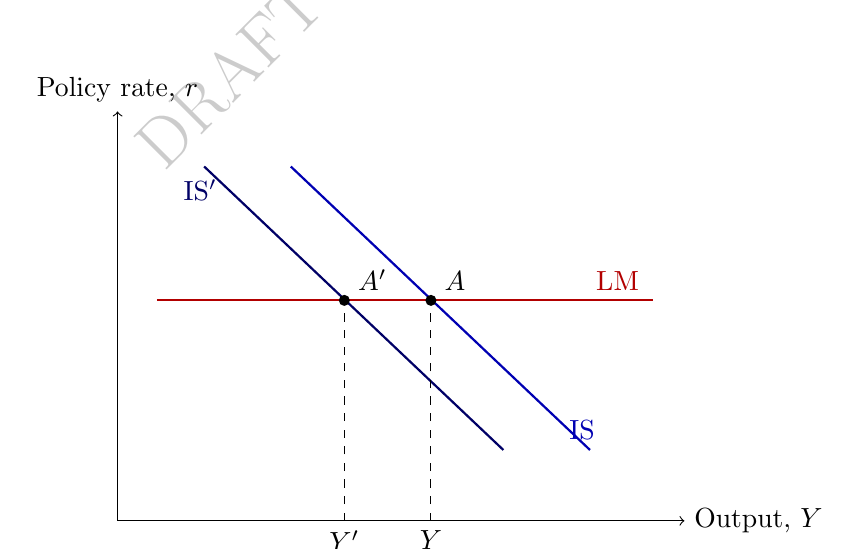
\begin{tikzpicture}[x=1cm,y=1cm]
\draw[->] (0,0) -- (7.2,0) node[right] {Output, $Y$};
\draw[->] (0,0) -- (0,5.2) node[above] {Policy rate, $r$};

% LM
\draw[thick,red!70!black] (0.5,2.8) -- (6.8,2.8);
\node[red!70!black] at (6.35,3.05) {LM};

% IS and IS'
\draw[thick,blue!70!black] (2.2,4.5) -- (6.0,0.9);
\node[blue!70!black] at (5.9,1.15) {IS};

\draw[thick,blue!40!black] (1.1,4.5) -- (4.9,0.9);
\node[blue!40!black] at (1.05,4.2) {IS$'$};

% Equilibria
\fill (3.98,2.8) circle (2pt);
\node[above right] at (4.03,2.8) {$A$};

\fill (2.88,2.8) circle (2pt);
\node[above right] at (2.93,2.8) {$A'$};

\draw[dashed] (3.98,0) -- (3.98,2.8);
\node[below] at (3.98,0) {$Y$};

\draw[dashed] (2.88,0) -- (2.88,2.8);
\node[below] at (2.88,0) {$Y'$};
\end{tikzpicture}
\end{center}

\noindent
An increase in $x$ shifts the IS curve left from IS to IS$'$, reducing equilibrium output from $Y$ to $Y'$.

\subsection{Policy responses to a financial shock}

Once a financial shock raises the risk premium, policymakers can respond through either fiscal policy or monetary policy.

\begin{definition}{Two main stabilization responses}{}
If the financial system becomes impaired and $x$ rises:
\begin{itemize}[leftmargin=1.5em]
    \item \textbf{Fiscal policy} can raise demand directly through $G\uparrow$ or $T\downarrow$.
    \item \textbf{Monetary policy} can lower the policy rate $r$ to reduce the borrowing rate $r+x$.
\end{itemize}
\end{definition}

\begin{theorem}{Offsetting a higher risk premium}{}
To keep the borrowing rate unchanged after a rise in the risk premium, the central bank must reduce the real policy rate one-for-one:
\[
\Delta(r+x)=0
\quad\Longrightarrow\quad
\Delta r = -\Delta x.
\]
\end{theorem}

\noindent
So if $x$ rises by $4$ percentage points, the central bank must reduce $r$ by $4$ percentage points to leave the borrowing rate unchanged.

\begin{examplebox}[title={Worked Example: Monetary offset of a financial shock}]
Suppose initially
\[
r=2\%, \qquad x=1\%,
\]
so the borrowing rate is
\[
r+x=3\%.
\]
Now suppose the risk premium rises by $4$ percentage points:
\[
x: 1\% \to 5\%.
\]
To keep the borrowing rate unchanged at $3\%$, the central bank must set
\[
r + 5\% = 3\%
\quad\Longrightarrow\quad
r=-2\%.
\]
Hence the real policy rate must fall from $2\%$ to $-2\%$.
\end{examplebox}

\begin{policynote}[title={Policy Application: Why the zero lower bound matters}]
Even if, in principle, monetary policy could offset a higher risk premium, it may be impossible in practice. Since
\[
r=i-\pi^e,
\]
the nominal interest rate required to achieve a sufficiently low real rate may have to be negative. If the nominal rate is stuck at the zero lower bound, the central bank may be unable to offset the shock fully, and a recession can still occur.
\end{policynote}

\subsection{Fiscal policy versus monetary policy in the extended model}

The extended model clarifies the different transmission channels:
\begin{itemize}[leftmargin=1.5em]
    \item \textbf{Fiscal policy} offsets weak private demand directly by shifting the IS curve right.
    \item \textbf{Monetary policy} works indirectly by reducing the real policy rate and therefore the borrowing rate.
    \item \textbf{Financial frictions} weaken monetary transmission because even if the policy rate falls, the borrowing rate may not fall much when $x$ rises sharply.
\end{itemize}

\begin{examtip}[title={Exam Focus: Transmission channels}]
In the extended IS--LM model:
\begin{itemize}[leftmargin=1.5em]
    \item policy rate $\downarrow \Rightarrow r\downarrow \Rightarrow r+x\downarrow \Rightarrow I\uparrow \Rightarrow Y\uparrow$;
    \item risk premium $\uparrow \Rightarrow r+x\uparrow \Rightarrow I\downarrow \Rightarrow Y\downarrow$;
    \item weak bank balance sheets often operate through \emph{higher} $x$ and weaker credit supply.
\end{itemize}
\end{examtip}

\subsection{Links back to the baseline IS--LM model}

\begin{theorem}{Baseline IS--LM as a special case}{}
The baseline IS--LM model is recovered as a special case of the extended model when:
\begin{itemize}[leftmargin=1.5em]
    \item expected inflation is ignored or fixed,
    \item the risk premium is zero or constant,
    \item all borrowing rates move one-for-one with the policy rate.
\end{itemize}
Then the relevant borrowing cost reduces to the single interest rate used in Lecture 3.
\end{theorem}

\noindent
The new content of Lecture 4 is therefore not a replacement of IS--LM, but an economically more realistic version of it.

\subsection{Worked example from Tutorial 4}

\begin{examplebox}[title={Worked Example (Tutorial 4, Question 4): True/false using the Fisher relation}]
Let $i$ denote the nominal interest rate, $r$ the real interest rate, and $\pi^e$ expected inflation. Recall:
\[
1+r=\frac{1+i}{1+\pi^e},
\qquad
r\approx i-\pi^e.
\]

\begin{enumerate}[label=(\alph*)]
    \item \textbf{Statement:} The nominal interest rate is measured in terms of goods; the real interest rate is measured in terms of money.

    \textbf{Answer: False.}  
    The nominal rate is measured in money terms, while the real rate is measured in goods or purchasing-power terms.

    \item \textbf{Statement:} As long as expected inflation remains roughly constant, movements in the real interest rate are roughly equal to movements in the nominal interest rate.

    \textbf{Answer: True.}  
    If $\pi^e$ is approximately constant, then from
    \[
    r\approx i-\pi^e
    \]
    it follows that
    \[
    \Delta r \approx \Delta i.
    \]

    \item \textbf{Statement:} When expected inflation increases, the real rate of interest falls.

    \textbf{Answer: Uncertain in general; true if the nominal rate is fixed.}  
    If $i$ is held fixed, then
    \[
    \pi^e\uparrow \Rightarrow r\downarrow.
    \]
    But if the central bank or market interest rates increase together with expected inflation, the real rate need not fall.

    \item \textbf{Statement:} The nominal policy interest rate is set by the central bank.

    \textbf{Answer: True.}  
    In the model, the central bank chooses the nominal policy rate and thereby influences the real policy rate.
\end{enumerate}
\end{examplebox}

\subsection{Short-run macroeconomic interpretation}

\begin{theorem}{Main macroeconomic lesson of the extended model}{}
A disturbance in the financial system can become a macroeconomic disturbance because it changes the borrowing rate faced by private agents. In particular:
\begin{itemize}[leftmargin=1.5em]
    \item weaker balance sheets and higher perceived risk increase the risk premium $x$;
    \item a higher $x$ raises borrowing costs and reduces investment;
    \item the IS curve shifts left and output falls;
    \item conventional monetary policy may be unable to offset this fully if the zero lower bound binds.
\end{itemize}
\end{theorem}

\begin{examtip}[title={Exam Focus: What Lecture 4 adds to Lecture 3}]
Lecture 3 said: the central bank sets the policy rate and this determines demand.  

Lecture 4 adds: the borrowing rate relevant for demand is
\[
r+x,
\]
not just the policy rate. Therefore financial stress can weaken demand even when monetary policy is unchanged or expansionary.
\end{examtip}


\newpage

%==================================================
% FILE: HE2002_RevisionNotes(2).tex
% REPLACE: section The Labor Market
%==================================================
\section{The Labor Market}

\subsection{Why the labour market matters for macroeconomics}

The labour market is the bridge between output and inflation. When firms increase production, they hire more workers; unemployment falls; workers bargain from a stronger position; nominal wages rise; firms raise prices; and prices feed back into wage claims. This wage--price interaction is why macroeconomics cannot stop at the goods market.

\begin{definition}{Labour-market categories}{}
Each person of working age is classified as:
\begin{itemize}[leftmargin=1.5em]
\item \textbf{Employed:} worked for pay or was temporarily absent from a job.
\item \textbf{Unemployed:} did not work but actively searched for work.
\item \textbf{Out of the labour force:} neither worked nor searched for work.
\end{itemize}
The \textbf{labour force} is the sum of employed and unemployed people.
\end{definition}

\begin{keyformula}[title={Key Formula: Core labour-market rates}]
\[
L=N+U,
\qquad
u=\frac{U}{L},
\qquad
\text{Participation rate}=\frac{L}{\text{working-age population}}.
\]
In Lecture 5, unemployment is the key summary statistic because it captures labour-market tightness and therefore wage pressure.
\end{keyformula}

\subsection{Stocks, flows, and labour-market tightness}

High unemployment matters on both margins:
\begin{itemize}[leftmargin=1.5em]
\item the employed face a higher probability of losing their jobs;
\item the unemployed face a lower probability of finding jobs.
\end{itemize}
So unemployment is not only a stock variable. It also summarises underlying \emph{flows} into and out of employment.

\begin{policynote}
In a recession, the labour market weakens twice over: job loss becomes more likely, and job finding becomes slower. This is why the unemployment rate is a central state variable later in the Phillips curve and IS--LM--PC framework.
\end{policynote}

\subsection{Wage determination}

\begin{definition}{Reservation wage and bargaining power}{}
The \textbf{reservation wage} is the wage that makes a worker indifferent between accepting a job and remaining unemployed. Actual wages are often above reservation wages because firms care about retention, morale, effort, and recruitment. Workers also have different bargaining power depending on outside options and labour-market conditions.
\end{definition}

Two facts matter for macro wage setting:
\begin{itemize}[leftmargin=1.5em]
\item wages usually exceed reservation wages;
\item wages are higher when unemployment is lower.
\end{itemize}

\begin{definition}{Efficiency wages}{}
Under \textbf{efficiency-wage} logic, firms may deliberately pay above-minimum wages because higher wages can raise productivity, reduce shirking, reduce turnover, and attract better workers.
\end{definition}

\begin{keyformula}[title={Key Formula: Wage-setting relation}]
\[
W=P^eF(u,z),
\qquad
\frac{\partial F}{\partial u}<0.
\]
Nominal wages depend positively on the expected price level $P^e$, negatively on unemployment $u$, and on a catch-all variable $z$ summarising institutions such as unemployment benefits, minimum-wage rules, and bargaining arrangements.
\end{keyformula}

\paragraph{Interpretation of the arguments.}
\begin{itemize}[leftmargin=1.5em]
\item \textbf{$P^e$:} workers care about the real wage, so higher expected prices induce higher nominal wage claims.
\item \textbf{$u$:} higher unemployment weakens bargaining power and lowers the wage consistent with wage setting.
\item \textbf{$z$:} stronger worker protection or more generous benefits raise wage pressure at a given unemployment rate.
\end{itemize}

\subsection{Price determination}

Lecture 5 uses a simple production structure:
\[
Y=AN.
\]
With the normalisation $A=1$, one worker produces one unit of output, so marginal cost is the nominal wage $W$.

\begin{keyformula}[title={Key Formula: Price-setting relation}]
\[
P=(1+m)W,
\qquad
\frac{W}{P}=\frac{1}{1+m}.
\]
The markup $m$ is the wedge between price and marginal cost. It determines the real wage firms are willing to pay.
\end{keyformula}

\begin{center}
\renewcommand{\arraystretch}{1.2}
\begin{tabularx}{\textwidth}{|p{2.2cm}|X|X|X|}
\hline
\textbf{Relation} & \textbf{Economic side} & \textbf{Slope / position} & \textbf{Main shifters} \\
\hline
WS & Workers and firms bargain over wages. & Downward sloping in $u$: weaker labour markets reduce the real wage sought in wage setting. & Expected prices and labour-market institutions $z$ \\
\hline
PS & Firms choose prices given marginal cost and markup. & Horizontal in the WS--PS diagram: the real wage implied by price setting is fixed at $1/(1+m)$. & Markup $m$ \\
\hline
\end{tabularx}
\end{center}

\subsection{Wage setting, price setting, and the natural rate}

If expected and actual prices coincide, $P^e=P$, then the wage-setting relation becomes
\[
\frac{W}{P}=F(u,z).
\]
This is the \textbf{WS relation}. It is downward sloping in unemployment.

The price-setting relation gives
\[
\frac{W}{P}=\frac{1}{1+m}.
\]
This is the \textbf{PS relation}. It is horizontal because the markup, not unemployment directly, pins down the real wage consistent with price setting.

\begin{center}
\begin{tikzpicture}[x=1cm,y=1cm]
\draw[->] (0,0) -- (8.2,0) node[right] {Unemployment rate, $u$};
\draw[->] (0,0) -- (0,5.2) node[above] {Real wage, $W/P$};

\draw[thick,blue!70!black] (0.7,4.4) .. controls (2.2,3.47) and (4.3,2.7) .. (7.1,1.1);
\node[blue!70!black] at (6.9,1.6) {WS};

\draw[thick,red!70!black] (0,2.3) -- (7.4,2.3);
\node[red!70!black] at (6.9,2.6) {PS};

\draw[dashed] (4.8,0) -- (4.8,2.3);
\fill (4.8,2.3) circle (2pt);
\node[above right] at (4.8,2.3) {$A$};
\node[below] at (4.8,0) {$u_n$};
\node[left] at (0,2.3) {$1/(1+m)$};
\end{tikzpicture}
\end{center}

\begin{theorem}{Natural rate of unemployment}{}
The natural rate of unemployment is the unemployment rate at which the real wage implied by wage setting equals the real wage implied by price setting:
\[
F(u_n,z)=\frac{1}{1+m}.
\]
At $u_n$, the labour market is in equilibrium in the WS--PS framework.
\end{theorem}

\begin{theorem}{Natural employment and natural output}{}
With $Y=N=L(1-u)$ in the course's simplified production structure,
\[
N_n=L(1-u_n),
\qquad
Y_n=N_n=L(1-u_n).
\]
So anything that raises $u_n$ lowers natural employment and natural output.
\end{theorem}

\subsection{Linear wage setting and the closed-form natural rate}

If
\[
F(u,z)=1-\alpha u+z,
\]
then the natural rate satisfies
\[
1-\alpha u_n+z=\frac{1}{1+m}.
\]

\begin{keyformula}[title={Key Formula: Closed-form natural rate}]
\[
u_n=\frac{1+z-\frac{1}{1+m}}{\alpha}
\approx \frac{m+z}{\alpha}.
\]
The approximation uses
\[
\frac{1}{1+m}\approx 1-m
\]
when the markup is not too large.
\end{keyformula}

\subsection{Comparative statics}

\paragraph{Higher wage pressure: $z\uparrow$.}
At a given unemployment rate, workers seek a higher real wage. WS shifts up, so the natural rate rises.

\paragraph{Higher markup: $m\uparrow$.}
A higher markup lowers the real wage firms are willing to pay:
\[
\frac{1}{1+m}\downarrow.
\]
PS shifts down, so the natural rate rises.

\begin{theorem}{The central comparative statics of Lecture 5}{}
\begin{itemize}[leftmargin=1.5em]
\item $z\uparrow \Rightarrow$ WS shifts up $\Rightarrow u_n\uparrow \Rightarrow Y_n\downarrow$.
\item $m\uparrow \Rightarrow$ PS shifts down $\Rightarrow u_n\uparrow \Rightarrow Y_n\downarrow$.
\end{itemize}
This is the logic later used for oil-price shocks and stagflation.
\end{theorem}

\begin{examplebox}[title={Worked Example: Natural unemployment with a higher markup}]
Suppose the markup is initially $m=0.05$ and the wage-setting equation is
\[
W=P(1-u).
\]
Then
\[
\frac{W}{P}=1-u.
\]
From price setting,
\[
\frac{W}{P}=\frac{1}{1.05}=\frac{20}{21}.
\]
So the natural rate satisfies
\[
1-u_n=\frac{20}{21}
\qquad\Rightarrow\qquad
u_n=\frac{1}{21}\approx 4.76\%.
\]

Now let the markup rise to $m=0.10$. Then
\[
\frac{W}{P}=\frac{1}{1.10}=\frac{10}{11},
\]
so
\[
1-u_n=\frac{10}{11}
\qquad\Rightarrow\qquad
u_n=\frac{1}{11}\approx 9.09\%.
\]

A higher markup raises the natural rate because firms are willing to pay a lower real wage, and a weaker labour market is needed to make that wage consistent with wage setting.
\end{examplebox}

\begin{commonmistake}
Do not say that unemployment directly shifts PS. In the course model, unemployment affects the \emph{wage-setting} relation. The price-setting relation shifts when the markup changes.
\end{commonmistake}

\begin{examtip}[title={Exam Focus: What you must be able to do quickly}]
You should be able to:
\begin{itemize}[leftmargin=1.5em]
\item explain why WS slopes downward and PS is horizontal;
\item derive $u_n$ from WS and PS;
\item explain how $z$ and $m$ shift the diagram;
\item connect a higher $u_n$ to lower natural employment and lower natural output;
\item recognise that Lecture 5 is the starting point for Chapters 6 and 7.
\end{itemize}
\end{examtip}




%==================================================
% FILE: HE2002_RevisionNotes(2).tex
% REPLACE: section The Phillips Curve, the Natural Rate of Unemployment, and Inflation
%==================================================
\section{The Phillips Curve, the Natural Rate of Unemployment, and Inflation}

\subsection{From wage setting to inflation}

Lecture 6 keeps the labour-market logic from Lecture 5, but no longer assumes that expected and actual prices must coincide when wages are set. Start from the linear wage-setting relation
\[
W=P^e(1-\alpha u+z)
\]
and the price-setting equation
\[
P=(1+m)W.
\]
Combining,
\[
P=P^e(1+m)(1-\alpha u+z).
\]

\begin{theorem}{Approximate derivation of the Phillips curve}{}
If the markup, the unemployment term, and the wage-setting term are not too large, then
\[
(1+m)(1-\alpha u+z)\approx 1+m-\alpha u+z.
\]
Hence
\[
\frac{P}{P^e}\approx 1+(m+z)-\alpha u.
\]
After expressing $P$ and $P^e$ relative to last period's price level, this becomes the expectations-augmented Phillips curve:
\[
\pi_t=\pi_t^e+(m+z)-\alpha u_t.
\]
\end{theorem}

\begin{keyformula}[title={Key Formula: Expectations-augmented Phillips curve}]
\[
\pi_t=\pi_t^e+(m+z)-\alpha u_t.
\]
This says:
\begin{itemize}[leftmargin=1.5em]
\item higher expected inflation raises actual inflation one-for-one;
\item higher markups raise inflation;
\item higher wage-setting pressure $z$ raises inflation;
\item higher unemployment lowers inflation.
\end{itemize}
\end{keyformula}

\subsection{The original Phillips curve}

If expected inflation is anchored at a constant value $\bar{\pi}$, then
\[
\pi_t=\bar{\pi}+(m+z)-\alpha u_t.
\]
This is the original Phillips curve: a stable negative relation between unemployment and inflation.

\begin{center}
\begin{tikzpicture}[x=1cm,y=0.8cm]
\draw[->] (0,0) -- (8.4,0) node[right] {Unemployment rate, $u$};
\draw[->] (0,-0.5) -- (0,5.3) node[above] {Inflation, $\pi$};
\draw[thick,blue!70!black] (0.8,4.5) -- (7.3,0.9);
\node[blue!70!black] at (6.6,2) {PC};
\draw[dashed] (4.9,0) -- (4.9,2.25);
\draw[dashed] (0,2.25) -- (4.9,2.25);
\fill (4.9,2.25) circle (2pt);
\node[below] at (4.9,0) {$u_n$};
\node[left] at (0,2.25) {$\pi^e$};
\end{tikzpicture}
\end{center}

The original interpretation suggested a stable inflation--unemployment trade-off. The central lesson of Lecture 6 is that this interpretation breaks down once expectations adjust.

\subsection{Expectation formation}

Lecture 6 uses the expectations rule
\[
\pi_t^e=(1-\theta)\bar{\pi}+\theta \pi_{t-1},
\]
where $\theta$ measures how much expected inflation depends on last period's actual inflation.

\begin{center}
\renewcommand{\arraystretch}{1.2}
\begin{tabularx}{\textwidth}{|p{1.8cm}|X|X|}
\hline
\textbf{Case} & \textbf{Interpretation} & \textbf{Implication for inflation dynamics} \\
\hline
$\theta=0$ & Fully anchored expectations & Inflation depends on unemployment relative to a fixed anchor $\bar{\pi}$. \\
\hline
$0<\theta<1$ & Partly adaptive expectations & Current inflation feeds partly into future inflation. Inflation persistence appears. \\
\hline
$\theta=1$ & Fully backward-looking expectations & Unemployment affects \emph{changes} in inflation rather than the inflation level. \\
\hline
\end{tabularx}
\end{center}

Substituting the expectations rule into the Phillips curve gives
\[
\pi_t=[(1-\theta)\bar{\pi}+(m+z)] + \theta\pi_{t-1}-\alpha u_t.
\]

\subsection{Accelerationist Phillips curve}

When $\theta=1$,
\[
\pi_t-\pi_{t-1}=(m+z)-\alpha u_t.
\]

\begin{keyformula}[title={Key Formula: Accelerationist Phillips curve}]
\[
\Delta\pi_t=(m+z)-\alpha u_t.
\]
Under fully adaptive expectations, unemployment below the natural rate leads to \emph{accelerating} inflation. Unemployment above the natural rate leads to \emph{decelerating} inflation.
\end{keyformula}

\subsection{The natural-rate form}

At the natural rate, actual inflation equals expected inflation. Set $\pi_t=\pi_t^e$ in
\[
\pi_t=\pi_t^e+(m+z)-\alpha u_t
\]
to obtain
\[
u_n=\frac{m+z}{\alpha}.
\]
Substituting back yields the most useful form of the Phillips curve:

\begin{keyformula}[title={Key Formula: Phillips curve around the natural rate}]
\[
\pi_t-\pi_t^e=-\alpha(u_t-u_n).
\]
Therefore:
\begin{itemize}[leftmargin=1.5em]
\item if $u_t=u_n$, inflation equals expected inflation;
\item if $u_t<u_n$, inflation is higher than expected;
\item if $u_t>u_n$, inflation is lower than expected.
\end{itemize}
\end{keyformula}

\begin{theorem}{What the natural rate means in Chapter 6}{}
The natural rate of unemployment is not zero unemployment and not ideal employment. It is the unemployment rate consistent with \emph{stable inflation}, in the sense that actual inflation equals expected inflation.
\end{theorem}

\subsection{A representative expectations example}

\begin{examplebox}[title={Worked Example: Holding unemployment below the natural rate}]
Suppose
\[
\pi_t=\pi_t^e+0.1-2u_t
\qquad\text{and}\qquad
\pi_t^e=(1-\theta)\bar{\pi}+\theta\pi_{t-1}.
\]
The natural rate solves
\[
0.1-2u_n=0
\qquad\Rightarrow\qquad
u_n=0.05=5\%.
\]

Now suppose policymakers hold unemployment at
\[
u=3\%=0.03<u_n.
\]

\paragraph{If $\theta=0$.}
Expected inflation remains fixed at $\bar{\pi}$. Then
\[
\pi_t=\bar{\pi}+0.1-2(0.03)=\bar{\pi}+0.04.
\]
So inflation jumps above the anchor by 4 percentage points, but does not keep rising further as long as expectations remain anchored.

\paragraph{If $\theta=1$.}
Expected inflation equals last period's inflation, so
\[
\pi_t-\pi_{t-1}=0.1-2(0.03)=0.04.
\]
Inflation rises by 4 percentage points every period. This is the accelerationist result.

\paragraph{Lesson.}
Trying to keep unemployment permanently below the natural rate is compatible with a one-off inflation increase only if expectations remain anchored. Once expectations become adaptive, inflation keeps accelerating.
\end{examplebox}

\subsection{Re-anchoring and historical interpretation}

The lecture's historical story can be summarised as follows:
\begin{itemize}[leftmargin=1.5em]
\item \textbf{1960s:} the original Phillips curve appeared stable.
\item \textbf{1970s--1980s:} expectations became more backward-looking; the accelerationist view became more relevant.
\item \textbf{Mid-1990s onward:} expectations in many advanced economies became more re-anchored around low inflation.
\end{itemize}

In the re-anchored period, the lecture writes a relation closer to
\[
\pi_t=\bar{\pi}+(m+z)-\alpha u_t.
\]
The fitted U.S. line shown in the lecture is
\[
\pi_t=2.8\%-0.16u_t.
\]

\subsection{Oil prices and the Phillips curve}

If an oil-price increase raises the markup $m$, then:
\begin{enumerate}[leftmargin=1.5em]
\item the Phillips curve shifts upward;
\item the natural rate of unemployment rises;
\item potential output later falls once we map unemployment into output.
\end{enumerate}
This is the bridge from Chapters 5--6 to the stagflation analysis in Chapter 7.

\begin{commonmistake}
Do not say ``low unemployment causes high inflation'' without stating the expectations regime. Under anchored expectations, low unemployment raises inflation relative to the anchor. Under the accelerationist Phillips curve, low unemployment raises the \emph{change} in inflation.
\end{commonmistake}

\begin{examtip}[title={Exam Focus: High-yield moves}]
You should be able to:
\begin{itemize}[leftmargin=1.5em]
\item derive or explain \(\pi_t=\pi_t^e+(m+z)-\alpha u_t\);
\item move from the inflation form to the natural-rate form;
\item distinguish anchored, partly adaptive, and fully adaptive expectations;
\item explain why the permanent inflation--unemployment trade-off disappears once expectations adjust.
\end{itemize}
\end{examtip}

%==================================================
% FILE: HE2002_RevisionNotes(2).tex
% REPLACE: section Lecture 7: From the Short to the Medium Run --- The IS--LM--PC Model
%==================================================
\newpage
\section{From the Short to the Medium Run --- The IS--LM--PC Model}

\subsection{The three-equation map}

Lecture 7 combines the demand side from IS--LM with the inflation side from Chapter 6. The model has three blocks:

\begin{center}
\renewcommand{\arraystretch}{1.2}
\begin{tabularx}{\textwidth}{|p{1.8cm}|p{4.7cm}|X|}
\hline
\textbf{Block} & \textbf{Equation} & \textbf{What it does} \\
\hline
IS & \(Y=C(Y-T)+I(Y,r+x)+G\) & Determines goods-market equilibrium for a given real policy rate and risk premium. \\
\hline
LM / policy & \(r=\bar r\) & The central bank chooses the real policy rate. \\
\hline
PC & \(\pi_t-\pi_t^e=-\alpha(u_t-u_n)\) & Links labour-market slack to inflation pressure. \\
\hline
\end{tabularx}
\end{center}

The missing step is that IS is written in output while the Phillips curve is written in unemployment. Chapter 7 therefore needs a bridge from unemployment to output.

\subsection{Okun's law as the bridge}

By definition,
\[
u=\frac{U}{L}=\frac{L-N}{L}=1-\frac{N}{L},
\]
so
\[
N=L(1-u).
\]
With the course's simplifying assumption $Y=N$,
\[
Y=L(1-u).
\]
At the natural rate,
\[
Y_n=L(1-u_n).
\]
Subtracting gives the course's Okun-type relation:

\begin{keyformula}[title={Key Formula: Output gap and unemployment gap}]
\[
Y-Y_n=-L(u-u_n).
\]
Hence:
\begin{itemize}[leftmargin=1.5em]
\item \(u=u_n \iff Y=Y_n\);
\item \(u>u_n \iff Y<Y_n\);
\item \(u<u_n \iff Y>Y_n\).
\end{itemize}
\end{keyformula}

Substituting into the Phillips curve:
\[
\pi-\pi^e=\frac{\alpha}{L}(Y-Y_n).
\]
If expectations are anchored at the central bank's target $\bar{\pi}$, then
\[
\pi-\bar{\pi}=\frac{\alpha}{L}(Y-Y_n).
\]

\subsection{Short-run output and inflation}

The Phillips curve is therefore upward sloping in output space: output above potential means inflation above target; output below potential means inflation below target.

\begin{center}
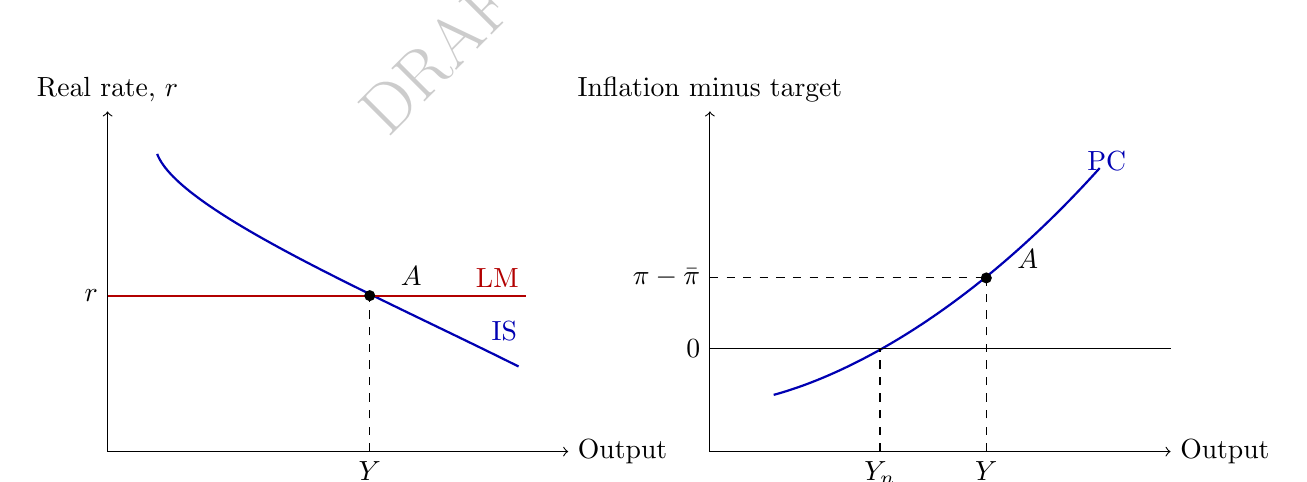
\begin{tikzpicture}[x=0.9cm,y=0.9cm]
% Left panel IS-LM
\begin{scope}[shift={(0,0)}]
\draw[->] (0,0) -- (6.5,0) node[right] {Output};
\draw[->] (0,0) -- (0,4.8) node[above] {Real rate, $r$};
\draw[thick,blue!70!black] (0.7,4.2) .. controls (1.0,3.4) and (3.8,2.2) .. (5.8,1.2);
\node[blue!70!black] at (5.6,1.7) {IS};
\draw[thick,red!70!black] (0,2.2) -- (5.9,2.2);
\node[red!70!black] at (5.5,2.45) {LM};
\node[left] at (0,2.2) {$r$};
\fill (3.7,2.2) circle (2pt);
\node[above right] at (4,2.2) {$A$};
\draw[dashed] (3.7,0) -- (3.7,2.2);
\node[below] at (3.7,0) {$Y$};
\end{scope}

% Right panel PC
\begin{scope}[shift={(8.5,0)}]
\draw[->] (0,0) -- (6.5,0) node[right] {Output};
\draw[->] (0,0) -- (0,4.8) node[above] {Inflation minus target};
\draw[thick,blue!70!black] (0.9,0.8) .. controls (2.0,1.1) and (3.7,2.0) .. (5.5,4.0);
\node[blue!70!black] at (5.6,4.1) {PC};
\draw[thin,black!70!black] (0,1.45) -- (6.5,1.45);
\node[left] at (0,2.45) {$\pi-\bar{\pi}$};
\node[left] at (0,1.45) {0};
\draw[dashed] (2.4,0) -- (2.4,1.45);
\draw[dashed] (0,1.45) -- (2.4,1.45);
\fill (3.9,2.45) circle (2pt);
\node[above right] at (4.2,2.45) {$A$};
\draw[dashed] (3.9,0) -- (3.9,2.45);
\draw[dashed] (0,2.45) -- (3.9,2.45);
\node[below] at (2.4,0) {$Y_n$};
\node[below] at (3.9,0) {$Y$};
\end{scope}
\end{tikzpicture}
\end{center}

At a low enough real policy rate, output rises above potential and inflation rises above target. This is the basic short-run overheating case.

\subsection{Medium-run equilibrium}

\begin{definition}{Natural rate of interest}{}
The \textbf{natural} or \textbf{neutral} real interest rate, denoted $r_n$, is the real rate consistent with
\[
Y=Y_n,\qquad u=u_n,\qquad \pi=\bar{\pi}.
\]
At this rate, the economy is at medium-run equilibrium with stable inflation.
\end{definition}

\begin{keyformula}[title={Key Formula: Medium-run equilibrium}]
\[
Y=Y_n,\qquad u=u_n,\qquad \pi=\bar{\pi},\qquad r=r_n.
\]
The borrowing rate relevant for spending is then
\[
r_n+x.
\]
If expected inflation is anchored at \(\bar{\pi}\), the corresponding nominal policy rate is
\[
i=r_n+\bar{\pi}.
\]
\end{keyformula}

\begin{theorem}{Why the medium run returns to potential}{}
If output differs from potential, inflation differs from target. As long as the central bank stabilises inflation, it has an incentive to adjust the real policy rate until the economy returns to
\[
Y=Y_n.
\]
So demand shocks create short-run deviations from potential, but not permanent ones.
\end{theorem}

\subsection{A useful shock taxonomy}

\begin{center}
\renewcommand{\arraystretch}{1.2}
\begin{tabularx}{\textwidth}{|p{3.1cm}|X|X|}
\hline
\textbf{Shock} & \textbf{Immediate model effect} & \textbf{Medium-run policy logic} \\
\hline
Fiscal contraction \(T\uparrow\) or \(G\downarrow\) & IS shifts left. At the initial rate, \(Y<Y_n\) and inflation falls below target. & The central bank lowers \(r\) until output returns to \(Y_n\). \\
\hline
Financial tightening \(x\uparrow\) & Borrowing rate \(r+x\) rises. IS shifts left and output falls. & The central bank can offset by lowering \(r\), but may be constrained by the zero lower bound. \\
\hline
Oil-price / markup shock \(m\uparrow\) & \(u_n\uparrow\), \(Y_n\downarrow\), and the Phillips curve shifts up. Inflation rises at the old output level. & The central bank must raise \(r\) if it wants inflation back at target. Output falls toward a lower potential level. \\
\hline
\end{tabularx}
\end{center}

\subsection{Diagnosing whether the economy is in medium-run equilibrium}

\begin{examplebox}[title={Worked Example: Medium-run checklist and central-bank response}]
Suppose
\[
Y_n=1000,\qquad u_n=5\%,\qquad r_n=2\%,\qquad x=1\%,\qquad \pi^e=2\%.
\]
Then the nominal policy rate consistent with medium-run equilibrium is
\[
i=r_n+\pi^e=4\%.
\]

\paragraph{Case A.}
If
\[
Y=1000,\quad u=5\%,\quad \pi=2\%,\quad i=4\%,\quad x=1\%,
\]
then
\[
r=i-\pi^e=4\%-2\%=2\%=r_n.
\]
All four medium-run conditions hold, so the economy is at medium-run equilibrium.

\paragraph{Case B.}
If
\[
Y=1050,\quad u=3\%,\quad \pi=3\%,\quad i=2\%,\quad x=1\%,
\]
then
\[
r=2\%-2\%=0\%<r_n.
\]
The borrowing rate is too low, demand is too strong, output is above potential, and inflation is above target. The central bank should \emph{raise} the policy rate.

\paragraph{Case C.}
If
\[
Y=950,\quad u=8\%,\quad \pi=1\%,\quad i=4\%,\quad x=3\%,
\]
then
\[
r=4\%-2\%=2\%=r_n,
\]
but the borrowing rate is
\[
r+x=5\%,
\]
which is above its natural level because the risk premium is high. This is a recession caused by tight financial conditions. The central bank can lower \(r\), and fiscal policy can also help.
\end{examplebox}

\subsection{Money neutrality in the medium run}

In medium-run steady state, the lecture writes money-market equilibrium as
\[
\frac{M}{P}=Y_nL(r_n+\bar{\pi}).
\]
If $Y_n$, $r_n$, and $\bar{\pi}$ are constant, real money demand is constant. Therefore real money supply must also be constant, which means that the price level must grow at the same rate as nominal money.

\begin{keyformula}[title={Key Formula: Money-growth result}]
If nominal money grows at rate \(g_M\), then in the medium run
\[
\pi=g_M,
\qquad
i=r_n+g_M.
\]
So money growth changes inflation and nominal rates, but not medium-run real output, unemployment, or the real interest rate.
\end{keyformula}

\subsection{The zero lower bound and deflation spirals}

The smooth medium-run adjustment can fail when the nominal interest rate is stuck at zero. Since
\[
r=i-\pi,
\]
if
\[
i=0
\qquad\text{and}\qquad
\pi<0,
\]
then
\[
r=-\pi>0.
\]
Deflation therefore \emph{raises} the real interest rate when the nominal rate cannot fall further.

\begin{policynote}[title={Policy Application: Deflation spiral}]
If inflation becomes negative while the nominal interest rate is at its lower bound, the real rate rises, output falls further below potential, and deflation pressure may intensify. This is the logic of the deflation spiral.
\end{policynote}

\begin{commonmistake}
A zero nominal interest rate does not automatically mean easy monetary policy. If inflation is sufficiently low or negative, the real rate may still be too high.
\end{commonmistake}

\newpage
\subsection{Fiscal consolidation revisited}

Suppose the economy starts at medium-run equilibrium and the government raises taxes to reduce its deficit.

\paragraph{Short run.}
Higher taxes shift IS left. At the initial real rate, output falls below potential and inflation falls below target.

\paragraph{Medium run.}
Because output is below potential and inflation is weak, the central bank lowers the real policy rate until output returns to $Y_n$.

\begin{examplebox}[title={Worked Example: Short-run versus medium-run effect of higher taxes}]
Initially,
\[
Y=Y_n,\qquad r=r_n,\qquad \pi=\bar{\pi}.
\]
Now let taxes increase.
\begin{enumerate}[leftmargin=1.5em]
\item IS shifts left, so at the original \(r_n\), output falls to \(Y'<Y_n\).
\item Because \(Y'<Y_n\), inflation falls below target.
\item The central bank lowers \(r\) until output returns to \(Y_n\).
\end{enumerate}
Result: output falls in the short run, but returns to potential in the medium run; the medium-run real interest rate is lower.
\end{examplebox}

\begin{policynote}
The composition result is important: in the medium run, fiscal consolidation lowers consumption but can raise investment through the lower interest rate. Output returns to potential, but its composition changes.
\end{policynote}

\newpage
\subsection{Oil-price increase and stagflation}

An increase in the real price of oil works like an increase in the markup \(m\):
\begin{enumerate}[leftmargin=1.5em]
\item in the labour market, PS shifts down, so \(u_n\) rises;
\item natural output falls because \(Y_n=L(1-u_n)\);
\item the Phillips curve shifts upward because inflation pressure is higher at each level of output.
\end{enumerate}

If the central bank does nothing, the economy stays at the old output level but with inflation above target. To prevent inflation from drifting upward and expectations from de-anchoring, the central bank raises the real rate. Output then falls toward the new, lower potential level.

\begin{center}
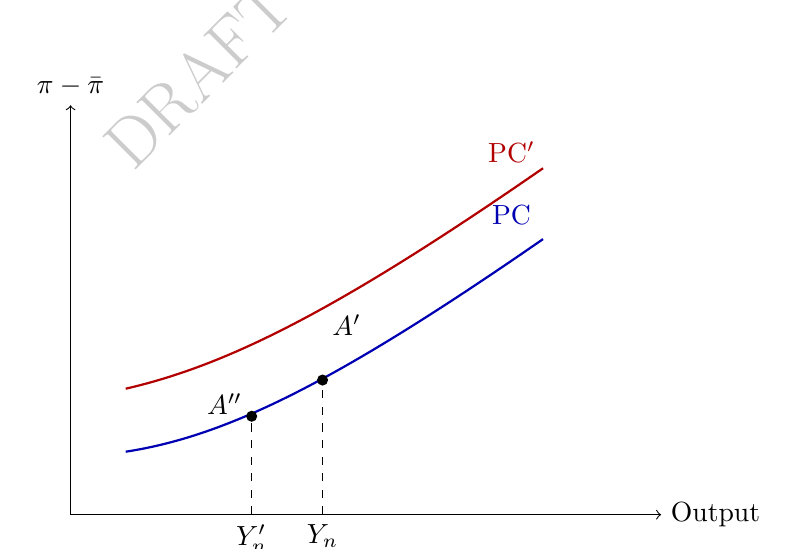
\begin{tikzpicture}[x=1cm,y=1cm]
\draw[->] (0,0) -- (7.5,0) node[right] {Output};
\draw[->] (0,0) -- (0,5.2) node[above] {$\pi-\bar{\pi}$};

\draw[thick,blue!70!black] (0.7,0.8) .. controls (2.0,1.0) and (3.4,1.7) .. (6.0,3.5);
\node[blue!70!black] at (5.6,3.8) {PC};

\draw[thick,red!70!black] (0.7,1.6) .. controls (2.0,1.9) and (3.4,2.6) .. (6.0,4.4);
\node[red!70!black] at (5.6,4.6) {PC$'$};

\draw[dashed] (3.2,0) -- (3.2,1.69);
\draw[dashed] (2.3,0) -- (2.3,1.19);
\node[below] at (3.2,0) {$Y_n$};
\node[below] at (2.3,0) {$Y_n'$};

\fill (3.2,1.71) circle (2pt);
\node[above right] at (3.2,2.15) {$A'$};
\fill (2.3,1.25) circle (2pt);
\node[above left] at (2.3,1.15) {$A''$};
\end{tikzpicture}
\end{center}

\begin{definition}{Stagflation}{}
\textbf{Stagflation} is the combination of lower output and higher inflation. In the chapter's framework, a permanent oil-price increase creates stagflation because it lowers potential output while shifting inflation pressure upward.
\end{definition}

\begin{examtip}[title={Exam Focus: Standard Chapter 7 script}]
For medium-run short answers, use the same five-step structure:
\begin{enumerate}[leftmargin=1.5em]
\item identify the shock;
\item state which equation or curve shifts;
\item describe the short-run effect at the initial policy rate;
\item explain why the central bank reacts;
\item state the new medium-run equilibrium.
\end{enumerate}
This script covers fiscal consolidation, financial shocks, and oil-price shocks.
\end{examtip}

%==================================================
% FILE: HE2002_RevisionNotes(2).tex
% REPLACE: section The Facts of Growth
%==================================================
\newpage
\section{The Facts of Growth}

\subsection{Why growth matters}

Growth is the sustained increase in output over time. For welfare, what matters is not just whether aggregate GDP rises, but whether output per person and output per worker rise in a persistent way.

\begin{definition}{Standard of living}{}
When comparing living standards across countries or across long periods of time, the most useful measure is \textbf{output per person}. When analysing production efficiency, the relevant measures are often \textbf{output per worker} or \textbf{output per hour worked}.
\end{definition}

Lecture 8 emphasises that, over long horizons, the welfare gains from sustained growth dominate the welfare gains from merely smoothing short-run fluctuations.

\subsection{What should be measured}

\begin{center}
\renewcommand{\arraystretch}{1.2}
\begin{tabularx}{\textwidth}{|p{3.0cm}|X|X|}
\hline
\textbf{Measure} & \textbf{Best use} & \textbf{Main trap} \\
\hline
Total output \(Y\) & Aggregate size of the economy & Large countries can have high GDP even if average living standards are modest. \\
\hline
Output per person \(Y/\text{population}\) & Living-standard comparison & Can differ from output per worker if participation differs. \\
\hline
Output per worker \(Y/N\) & Production efficiency and growth modelling & Says less directly about welfare if employment rates differ strongly across countries. \\
\hline
PPP-adjusted output per person & Cross-country welfare comparison & Must not be confused with values converted using market exchange rates. \\
\hline
\end{tabularx}
\end{center}

\subsection{PPP and international comparisons}

Market exchange rates can give a misleading picture of relative living standards because prices differ across countries. Cross-country comparisons therefore use \textbf{purchasing power parity (PPP)}.

\begin{definition}{Purchasing power parity}{}
PPP values output or expenditure using a common set of prices, so that measured differences reflect differences in quantities rather than local price levels.
\end{definition}

\begin{examplebox}[title={Worked Example: Exchange-rate comparison versus PPP}]
Suppose the average student in Japan buys 60 units of food at \yen 600 each and 80 transportation services at \yen 170 each. Monthly Japanese consumption is
\[
600\times 60 + 170\times 80 = 49{,}600 \text{ yen}.
\]

Suppose the average student in China buys 50 units of food at RMB15 each and 100 transportation services at RMB3 each. Monthly Chinese consumption is
\[
15\times 50 + 3\times 100 = 1{,}050 \text{ yuan}.
\]

If the market exchange rate is 1 yuan = 17 yen, Chinese consumption converted at market exchange rates is
\[
1{,}050\times 17 = 17{,}850 \text{ yen}.
\]

But if the Chinese bundle is valued at Japanese prices, PPP consumption is
\[
600\times 50 + 170\times 100 = 47{,}000 \text{ yen}.
\]

The lesson is that market exchange rates can understate real living standards in relatively cheap economies.
\end{examplebox}

\subsection{Stylised facts about growth}

Lecture 8 highlights several broad facts:
\begin{enumerate}[leftmargin=1.5em]
\item sustained increases in output per person are historically recent;
\item the post-1950 era saw strong growth in rich economies;
\item convergence is clearer among relatively similar rich economies than across the world as a whole;
\item growth experiences differ sharply across regions because institutions, conflict, education, and technology adoption differ.
\end{enumerate}

\begin{definition}{Convergence}{}
\textbf{Convergence} means poorer economies tending to grow faster than richer ones, thereby catching up in levels of output per person.
\end{definition}

\begin{definition}{Malthusian trap}{}
A \textbf{Malthusian trap} is a regime in which productivity improvements are too weak to produce sustained increases in output per person, so living standards remain broadly stagnant over long periods.
\end{definition}

\begin{theorem}{Why convergence is not universal}{}
Convergence is not a mechanical law saying that every poor country must catch up. It is at best \textbf{conditional}: countries converge more readily when institutions, education, saving behaviour, and access to technology support catch-up growth.
\end{theorem}

\newpage
\subsection{The production side of growth}

Lecture 8 introduces the aggregate production function
\[
Y=F(K,N).
\]

\begin{definition}{Constant returns to scale}{}
The production function has \textbf{constant returns to scale} if multiplying all inputs by the same factor multiplies output by that same factor:
\[
F(xK,xN)=xF(K,N).
\]
\end{definition}

With constant returns to scale,
\[
\frac{Y}{N}=F\!\left(\frac{K}{N},1\right)=f\!\left(\frac{K}{N}\right).
\]
So output per worker depends on capital per worker.

\begin{center}
\begin{tikzpicture}[x=1cm,y=1cm]
\draw[->] (0,0) -- (7.8,0) node[right] {Capital per worker, $K/N$};
\draw[->] (0,0) -- (0,5.2) node[above] {Output per worker, $Y/N$};

\draw[thick,blue!70!black] (0.5,0.6) .. controls (1.8,2.4) and (3.1,3.5) .. (7.0,4.5);
\node[blue!70!black] at (6.5,3.7) {$f(K/N)$};

\draw[thick,red!70!black,dashed] (0.5,1.2) .. controls (1.8,3.0) and (3.1,4.1) .. (7.0,5.0);
\node[red!70!black] at (6.2,5.05) {$f'(K/N)$};
\end{tikzpicture}
\end{center}

The solid curve is the production function. The dashed upward shift represents technological progress. Growth in output per worker can therefore come from:
\begin{itemize}[leftmargin=1.5em]
\item moving \emph{along} a given production function through higher capital per worker;
\item shifting the entire production function upward through better technology.
\end{itemize}

\begin{theorem}{Core growth result of Lecture 8}{}
Capital accumulation can raise output per worker, but because of diminishing returns it cannot sustain permanent growth in output per worker by itself. Sustained long-run growth requires technological progress.
\end{theorem}

\begin{commonmistake}
Do not equate GDP growth with rising living standards. Population growth can make total output rise even when output per person changes little.
\end{commonmistake}

\begin{examtip}[title={Exam Focus: What to prioritise from Chapter 8}]
Be ready to explain:
\begin{itemize}[leftmargin=1.5em]
\item why PPP is preferred to market exchange rates for living-standard comparisons;
\item what convergence means and why it is conditional rather than automatic;
\item why capital accumulation moves the economy \emph{along} the production function while technology shifts the function upward.
\end{itemize}
\end{examtip}

%==================================================
% FILE: HE2002_RevisionNotes(2).tex
% REPLACE: section Saving, Capital Accumulation, and Output
%==================================================
\newpage
\section{Saving, Capital Accumulation, and Output}

\subsection{The core feedback loop}

Lecture 9 formalises the circular mechanism
\[
K \Rightarrow Y \Rightarrow S \Rightarrow I \Rightarrow \Delta K.
\]
Capital determines output, output determines saving and investment, and investment determines future capital.

Assume no technological progress and a constant labour force \(N\). Define
\[
y_t=\frac{Y_t}{N},
\qquad
k_t=\frac{K_t}{N}.
\]
Then
\[
y_t=f(k_t).
\]

\subsection{Saving and capital accumulation}

The lecture makes three simplifying assumptions:
\begin{enumerate}[leftmargin=1.5em]
\item the economy is closed;
\item public saving is zero, so \(T-G=0\);
\item private saving is proportional to income: \(S=sY\).
\end{enumerate}
Thus
\[
I_t=sY_t.
\]
Capital evolves according to
\[
K_{t+1}=(1-\delta)K_t+I_t.
\]
Dividing by \(N\) gives
\[
k_{t+1}-k_t=s f(k_t)-\delta k_t.
\]

\begin{keyformula}[title={Key Formula: Law of motion for capital per worker}]
\[
k_{t+1}-k_t=s f(k_t)-\delta k_t.
\]
Capital per worker rises when investment per worker exceeds depreciation per worker, and falls when the reverse is true.
\end{keyformula}

\newpage
\subsection{Steady state}

\begin{definition}{Steady state without technological progress}{}
A \textbf{steady state} is a position in which capital per worker and output per worker are constant over time. Therefore
\[
k_{t+1}=k_t=k^*
\]
and the steady-state condition is
\[
s f(k^*)=\delta k^*.
\]
\end{definition}

\begin{center}
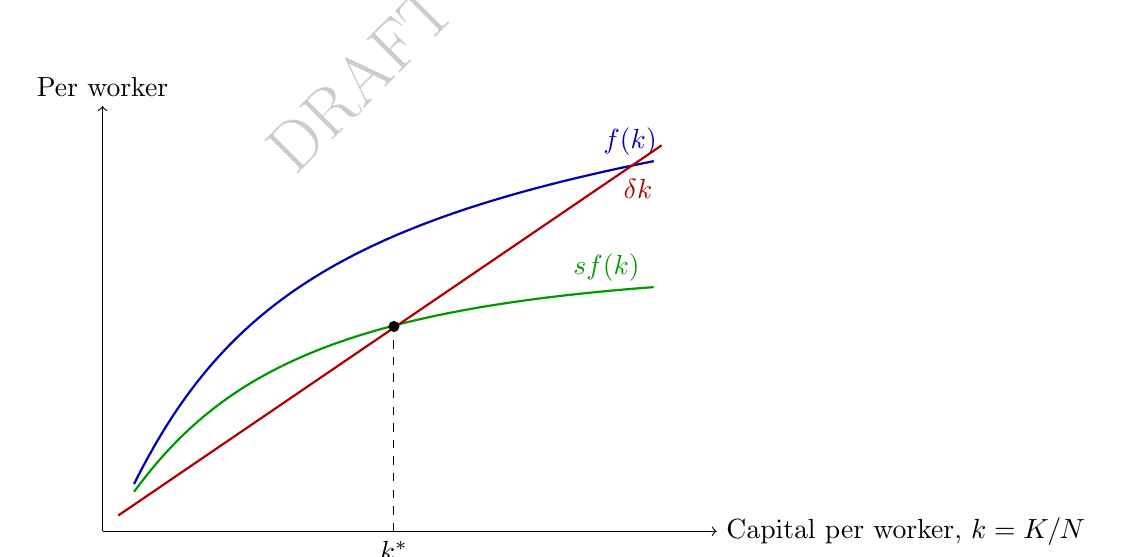
\begin{tikzpicture}[x=1cm,y=1cm]
\draw[->] (0,0) -- (7.8,0) node[right] {Capital per worker, $k=K/N$};
\draw[->] (0,0) -- (0,5.4) node[above] {Per worker};

\draw[thick,blue!70!black] (0.4,0.6) .. controls (1.5,2.8) and (3.0,3.9) .. (7.0,4.7);
\node[blue!70!black] at (6.7,4.95) {$f(k)$};

\draw[thick,green!60!black] (0.4,0.5) .. controls (1.5,2) and (3.0,2.8) .. (7.0,3.1);
\node[green!60!black] at (6.4,3.35) {$sf(k)$};

\draw[thick,red!70!black] (0.2,0.2) -- (7.1,4.9);
\node[red!70!black] at (6.8,4.35) {$\delta k$};

\fill (3.7,2.6) circle (2pt);
\draw[dashed] (3.7,0) -- (3.7,2.6);
\node[below] at (3.7,0) {$k^*$};
\end{tikzpicture}
\end{center}

\begin{theorem}{Direction of motion around the steady state}{}
\begin{itemize}[leftmargin=1.5em]
\item If \(sf(k)>\delta k\), then \(k\) rises.
\item If \(sf(k)<\delta k\), then \(k\) falls.
\item At \(sf(k)=\delta k\), the economy is at steady state.
\end{itemize}
\end{theorem}

\subsection{Effects of a higher saving rate}

A higher saving rate shifts the \(sf(k)\) curve upward. The new steady state has higher capital per worker and higher output per worker.

\begin{theorem}{Level effect of the saving rate}{}
In the model without technological progress, a higher saving rate raises the \emph{steady-state level} of output per worker, but not the \emph{steady-state growth rate} of output per worker. The long-run growth rate of output per worker remains zero.
\end{theorem}

So a rise in saving generates higher growth only during the transition to the new steady state.

\newpage
\subsection{Golden-rule capital}

People care about consumption, not output alone. In steady state,
\[
c^*=y^*-\delta k^*=f(k^*)-\delta k^*.
\]

\begin{definition}{Golden-rule level of capital}{}
The \textbf{golden-rule} level of capital is the level of steady-state capital that maximises steady-state consumption per worker.
\end{definition}

\begin{theorem}{Golden-rule condition}{}
In the basic Solow model without technological progress, steady-state consumption is maximised when
\[
f'(k_{GR})=\delta.
\]
So the marginal product of capital at the golden-rule capital stock equals the depreciation rate.
\end{theorem}

\noindent
This condition is the most general way to recognise golden-rule capital. If the economy saves too little, raising the saving rate increases steady-state consumption. If it saves too much, further increases in saving lower steady-state consumption because too much output is absorbed by maintaining a large capital stock.

\begin{commonmistake}
The golden rule does \emph{not} maximise output per worker. It maximises \emph{consumption per worker in steady state}.
\end{commonmistake}

\subsection{Worked magnitudes under the square-root production function}

Lecture 9 uses
\[
Y=K^{1/2}N^{1/2},
\qquad\text{so}\qquad
y=\sqrt{k}.
\]
Then the law of motion is
\[
k_{t+1}-k_t=s\sqrt{k_t}-\delta k_t.
\]

At steady state,
\[
s\sqrt{k^*}=\delta k^*.
\]
For \(k^*>0\), divide by \(\sqrt{k^*}\):
\[
s=\delta\sqrt{k^*}
\qquad\Rightarrow\qquad
k^*=\left(\frac{s}{\delta}\right)^2,
\qquad
y^*=\frac{s}{\delta}.
\]

\begin{examplebox}[title={Worked Example: Consumption and the golden rule in the square-root case}]
Using
\[
y^*=\frac{s}{\delta}
\qquad\text{and}\qquad
k^*=\left(\frac{s}{\delta}\right)^2,
\]
steady-state consumption per worker is
\[
c^*=y^*-\delta k^*
=\frac{s}{\delta}-\delta\left(\frac{s}{\delta}\right)^2
=\frac{s(1-s)}{\delta}.
\]
This is maximised when \(s=\tfrac12\). So in this special case, the golden-rule saving rate is 50\%.
\end{examplebox}

\subsection{Human capital}

Lecture 9 extends the production side to include human capital \(H\):
\[
\frac{Y}{N}=f\!\left(\frac{K}{N},\frac{H}{N}\right).
\]
Education, training, and organisational know-how can raise output per worker just as physical capital can.

\begin{policynote}
The parallel conclusion for physical and human capital is central:
\begin{itemize}[leftmargin=1.5em]
\item more physical or human capital can raise the \emph{level} of output per worker;
\item given the rate of technological progress, neither by itself produces permanently faster long-run growth.
\end{itemize}
\end{policynote}

\begin{examtip}[title={Exam Focus: Standard Solow answer}]
For Chapter 9, a strong short answer usually does four things:
\begin{enumerate}[leftmargin=1.5em]
\item writes the law of motion;
\item states the steady-state condition;
\item shows the relevant diagrammatic shift;
\item explains whether the effect is on a level or on a growth rate.
\end{enumerate}
\end{examtip}

%==================================================
% FILE: HE2002_RevisionNotes(2).tex
% REPLACE: section Technological Progress and Growth
%==================================================
\newpage
\section{Technological Progress and Growth}

\subsection{Why technology must enter the model}

Chapter 9 showed that without technological progress, output per worker eventually stops growing. Chapter 10 therefore introduces technology explicitly.

\begin{definition}{Extended production function}{}
Let \(A\) denote the state of technology. The lecture uses
\[
Y=F(K,AN),
\]
where \(AN\) is \textbf{effective labour}.
\end{definition}

\paragraph{Intuition of effective labour.}
If technology doubles, a given number of workers becomes twice as productive. It is as if the economy had twice as many workers in efficiency terms. That is why output is produced using capital \(K\) and effective labour \(AN\).

\subsection{Per-effective-worker variables}

With constant returns to scale,
\[
\frac{Y}{AN}=f\!\left(\frac{K}{AN}\right).
\]
Define
\[
\tilde{y}=\frac{Y}{AN},
\qquad
\tilde{k}=\frac{K}{AN}.
\]
Then
\[
\tilde{y}=f(\tilde{k}).
\]

\begin{keyformula}[title={Key Formula: The right unit of analysis}]
\[
\tilde{y}=f(\tilde{k}),
\qquad
\tilde{k}=\frac{K}{AN}.
\]
Once technology is growing, steady-state analysis must be done \emph{per effective worker}, not merely per worker.
\end{keyformula}

\subsection{Required investment with technology and labour-force growth}

Let technology grow at rate \(g_A\) and labour grow at rate \(g_N\):
\[
A_{t+1}=(1+g_A)A_t,
\qquad
N_{t+1}=(1+g_N)N_t.
\]
To keep capital per effective worker constant, investment must:
\begin{itemize}[leftmargin=1.5em]
\item replace depreciated capital;
\item equip new workers;
\item equip the higher level of effective labour created by technological progress.
\end{itemize}

\begin{keyformula}[title={Key Formula: Required investment}]
\[
I_R=(\delta+g_A+g_N)K.
\]
Therefore, in per-effective-worker terms,
\[
\frac{I_R}{AN}=(\delta+g_A+g_N)\tilde{k}.
\]
\end{keyformula}

\subsection{The dynamic equation in per-effective-worker terms}

Since saving is still \(I=sY\), actual investment per effective worker is
\[
\frac{I}{AN}=s f(\tilde{k}).
\]

\begin{keyformula}[title={Key Formula: Law of motion with technological progress}]
\[
\tilde{k}_{t+1}-\tilde{k}_t=s f(\tilde{k}_t)-(\delta+g_A+g_N)\tilde{k}_t.
\]
This is the exact analogue of the Chapter 9 law of motion, but written in per-effective-worker terms.
\end{keyformula}

\subsection{Steady state with technology}

A steady state in per-effective-worker terms requires
\[
\tilde{k}_{t+1}=\tilde{k}_t=\tilde{k}^*,
\]
so
\[
s f(\tilde{k}^*)=(\delta+g_A+g_N)\tilde{k}^*.
\]

\begin{center}
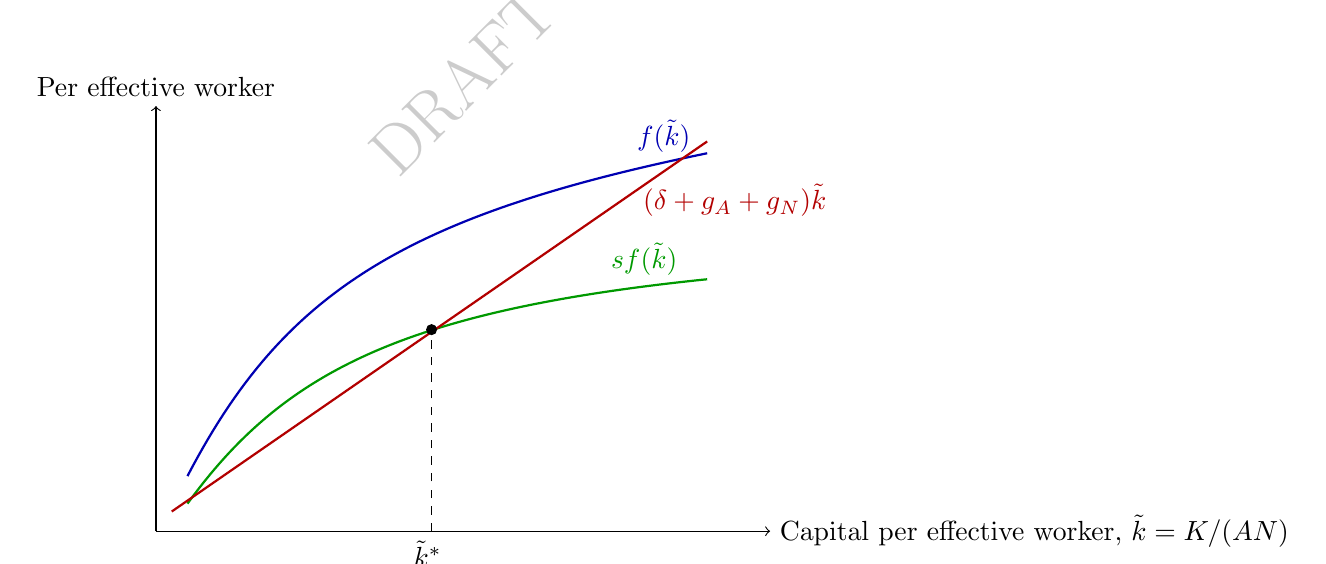
\begin{tikzpicture}[x=1cm,y=1cm]
\draw[->] (0,0) -- (7.8,0) node[right] {Capital per effective worker, $\tilde{k}=K/(AN)$};
\draw[->] (0,0) -- (0,5.4) node[above] {Per effective worker};

\draw[thick,blue!70!black] (0.4,0.7) .. controls (1.6,3.0) and (3.1,4.0) .. (7.0,4.8);
\node[blue!70!black] at (6.45,5.02) {$f(\tilde{k})$};

\draw[thick,green!60!black] (0.4,0.35) .. controls (1.6,2.0) and (3.1,2.8) .. (7.0,3.2);
\node[green!60!black] at (6.2,3.45) {$sf(\tilde{k})$};

\draw[thick,red!70!black] (0.2,0.25) -- (7.0,4.95);
\node[red!70!black] at (7.35,4.2) {$(\delta+g_A+g_N)\tilde{k}$};

\fill (3.5,2.56) circle (2pt);
\draw[dashed] (3.5,0) -- (3.5,2.56);
\node[below] at (3.45,0) {$\tilde{k}^*$};
\end{tikzpicture}
\end{center}

\begin{definition}{Balanced growth path}{}
The steady state of the technology-augmented model is called a \textbf{balanced growth path}. Along it, \(\tilde{k}\) and \(\tilde{y}\) are constant even though total output, total capital, and output per worker continue to grow.
\end{definition}

\subsection{Growth rates on the balanced growth path}

If \(\tilde{k}\) and \(\tilde{y}\) are constant in steady state, then
\[
g_K=g_Y=g_A+g_N.
\]
Output per worker grows at
\[
g_{Y/N}=g_A.
\]

\begin{theorem}{Long-run growth result}{}
On the balanced growth path:
\begin{align*}
g_K &= g_Y = g_A+g_N,\\
g_{K/N} &= g_{Y/N} = g_A,\\
g_{\tilde{k}} &= g_{\tilde{y}} = 0.
\end{align*}
So technological progress is the source of sustained growth in output per worker.
\end{theorem}

\subsection{A representative steady-state example}

\begin{examplebox}[title={Worked Example: Steady state with technology and population growth}]
Suppose
\[
Y=K^{1/2}(AN)^{1/2},
\qquad
s=0.16,
\qquad
\delta=0.10,
\qquad
g_A=0.04,
\qquad
g_N=0.02.
\]
Then
\[
\tilde{y}=\tilde{k}^{1/2}.
\]
The steady-state condition is
\[
0.16\sqrt{\tilde{k}^*}=(0.10+0.04+0.02)\tilde{k}^*.
\]
Since
\[
\delta+g_A+g_N=0.16,
\]
we obtain
\[
\sqrt{\tilde{k}^*}=1
\qquad\Rightarrow\qquad
\tilde{k}^*=1,
\qquad
\tilde{y}^*=1.
\]

The steady-state growth rates are:
\[
g_{\tilde{y}}=0,
\qquad
g_{Y/N}=g_A=4\%,
\qquad
g_Y=g_A+g_N=6\%.
\]

This example is useful because it cleanly separates:
\begin{itemize}[leftmargin=1.5em]
\item zero growth \emph{per effective worker},
\item positive growth \emph{per worker},
\item even faster growth of \emph{total output} when population also grows.
\end{itemize}
\end{examplebox}

\subsection{What a higher saving rate can and cannot do}

A higher saving rate shifts \(sf(\tilde{k})\) upward and raises the steady-state \emph{level} of output per effective worker. It also raises the level of output per worker. But it does \emph{not} change the long-run growth rate:
\[
g_{Y/N}=g_A.
\]

\begin{commonmistake}
A higher saving rate changes the steady-state \emph{level} of output per worker, not the permanent growth rate of output per worker. The permanent growth rate is pinned down by \(g_A\), not by \(s\).
\end{commonmistake}

\begin{commonmistake}
Do not forget why the required-investment line is
\[
(\delta+g_A+g_N)\tilde{k}.
\]
It includes replacement of worn-out capital, population growth, and the need to equip more efficient workers.
\end{commonmistake}

\subsection{Determinants of technological progress}

The later part of Chapter 10 is more conceptual and is best revised as a concept map rather than a derivation bank.

\begin{examtip}[title={Exam Focus: Likely MCQ-only}]
The lecture material on R\&D, patents, institutions, and frontier versus follower growth is most efficiently revised through contrasts and key definitions rather than full algebra.
\end{examtip}

\paragraph{Research and development.}
Most technological progress comes from firms' R\&D activity. Two ideas are central:
\begin{itemize}[leftmargin=1.5em]
\item \textbf{Fertility of research:} how effectively research inputs generate ideas.
\item \textbf{Appropriability:} how much of the return to innovation can be captured by innovators.
\end{itemize}

\paragraph{Patent laws.}
Patents strengthen incentives to innovate but can slow diffusion if protection is too strong. Good patent design balances incentives and diffusion.

\paragraph{Innovation versus imitation.}
Countries near the world technology frontier must innovate. Countries far behind can grow rapidly by imitating and adapting existing technologies.

\paragraph{Institutions and property rights.}
Innovation and investment depend on an institutional environment that protects property rights, enforces contracts, and supports competition and knowledge diffusion.

\begin{policynote}
The long-run message is that prosperity depends not only on capital accumulation but also on research incentives, institutions, and the ability to diffuse and use ideas productively.
\end{policynote}

\begin{examtip}[title={Exam Focus: High-yield analytical core}]
For the short-answer part of Chapter 10, prioritise:
\begin{itemize}[leftmargin=1.5em]
\item the meaning of effective labour;
\item the law of motion in per-effective-worker terms;
\item the required-investment line \((\delta+g_A+g_N)\tilde{k}\);
\item why output per worker grows at \(g_A\) on the balanced growth path.
\end{itemize}
\end{examtip}

%==================================================
% FILE: HE2002_RevisionNotes(2).tex
% REPLACE: section The Challenges of Growth
%==================================================
\newpage
\section{The Challenges of Growth}

Lecture 11 is more qualitative than the earlier growth chapters. The efficient way to revise it is to organise the material around contrasts, definitions, and policy logic.

\begin{examtip}[title={Exam Focus: Likely MCQ-only}]
For Chapter 11, the most examinable material is usually recognition-based:
\begin{itemize}[leftmargin=1.5em]
\item automation versus new-task creation;
\item growth versus inequality;
\item externalities versus carbon pricing.
\end{itemize}
\end{examtip}

\subsection{Robots, AI, and unemployment}

The crude claim that technological progress must permanently raise unemployment is too strong. Historically, advanced economies have experienced rising productivity without any sustained upward trend in aggregate unemployment.

\begin{definition}{Tasks, not jobs}{}
A useful way to think about automation is that technology replaces \emph{tasks}, not entire jobs. Jobs are bundles of tasks. Some tasks disappear, some remain, and new tasks may be created.
\end{definition}

The lecture frames the labour-market effect of AI as a balance between:
\begin{enumerate}[leftmargin=1.5em]
\item the \textbf{automation effect}: machines replace labour in existing tasks;
\item the \textbf{new-task effect}: new activities and occupations emerge, creating labour demand.
\end{enumerate}

\begin{policynote}
The cautious conclusion is not that AI must create mass permanent unemployment. It is that AI can strongly reshape the \emph{composition} of employment, wages, and skill demand even if aggregate employment eventually recovers.
\end{policynote}

\subsection{Creative destruction and inequality}

\begin{definition}{Creative destruction}{}
\textbf{Creative destruction} is the process by which new technologies, firms, and production methods displace old ones. It is central to long-run growth but also creates transitional disruption.
\end{definition}

Lecture 11 emphasises three dimensions of inequality:
\begin{itemize}[leftmargin=1.5em]
\item \textbf{Skill inequality:} technological progress may complement skilled labour more than unskilled labour.
\item \textbf{Trade-related pressure:} low-skill wages may be compressed when domestic firms face competition from low-wage producers abroad.
\item \textbf{Top-income inequality:} capital income and capital gains matter heavily at the very top of the distribution.
\end{itemize}

\begin{definition}{Skill-biased technological progress}{}
\textbf{Skill-biased technological progress} refers to innovations that raise the productivity and wages of more educated or more adaptable workers relatively more than those of less skilled workers.
\end{definition}

\subsection{Lorenz curve and the Gini coefficient}

\begin{definition}{Gini coefficient}{}
The \textbf{Gini coefficient} is a summary measure of income inequality ranging from 0 (perfect equality) to 1 (perfect inequality).
\end{definition}

\begin{center}
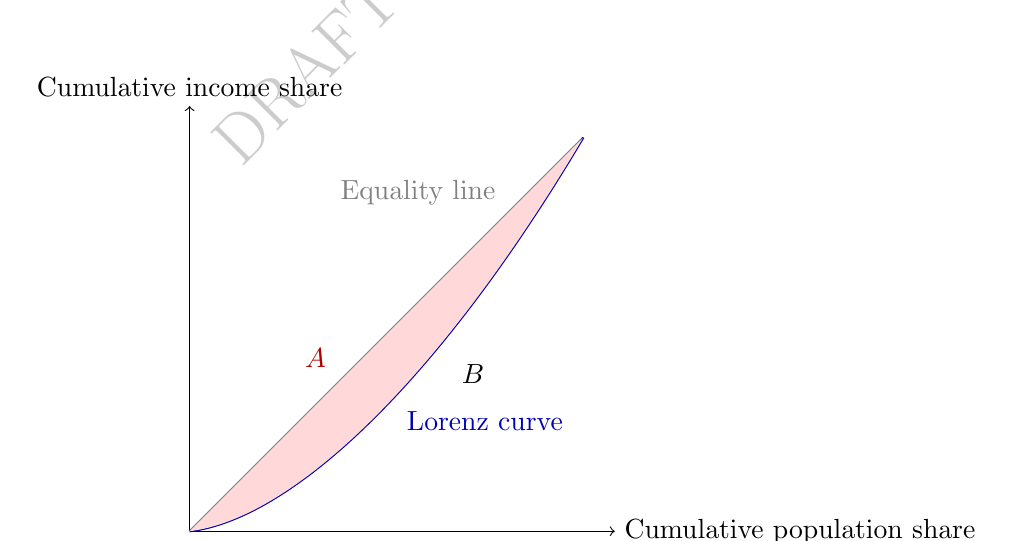
\begin{tikzpicture}[x=5cm,y=5cm]
\draw[->] (0,0) -- (1.08,0) node[right] {Cumulative population share};
\draw[->] (0,0) -- (0,1.08) node[above] {Cumulative income share};

\draw[thick,gray] (0,0) -- (1,1);
\node[gray] at (0.58,0.86) {Equality line};

\draw[thick,blue!70!black] (0,0) .. controls (0.25,0.03) and (0.62,0.36) .. (1,1);
\node[blue!70!black] at (0.75,0.28) {Lorenz curve};

\fill[red!15] (0,0) -- (1,1) .. controls (0.62,0.36) and (0.25,0.03) .. cycle;
\node[red!70!black] at (0.32,0.44) {$A$};
\node at (0.72,0.40) {$B$};
\end{tikzpicture}
\end{center}

Using the Lorenz-curve geometry from the lecture,
\[
\text{Gini}=\frac{A}{A+B}.
\]

\begin{commonmistake}
A higher Gini means \emph{more} inequality, not more equality. Also, the Gini is only a summary statistic: it does not by itself tell you where in the income distribution the inequality is concentrated.
\end{commonmistake}

\subsection{Redistribution and inclusive growth}

Governments can reduce inequality in two broad ways:
\begin{itemize}[leftmargin=1.5em]
\item reduce \textbf{market-income inequality} through education, labour-market policy, or wage-setting institutions;
\item reduce \textbf{disposable-income inequality} through taxes and transfers.
\end{itemize}

\begin{definition}{Market income and disposable income}{}
\textbf{Market income} is income before taxes and government transfers.  
\textbf{Disposable income} is income after taxes and transfers.
\end{definition}

The lecture's comparative evidence across OECD countries emphasises that countries differ not only in market inequality, but also in how much redistribution they undertake.

\subsection{Climate change as an externality}

\begin{definition}{Externality}{}
An \textbf{externality} arises when the action of a firm or household affects others without that effect being fully reflected in market prices.
\end{definition}

Climate change is a major growth-related externality because fossil-fuel use raises greenhouse-gas emissions, while the social damage is not fully priced by private decision makers.

\begin{definition}{Carbon pricing}{}
\textbf{Carbon pricing} means making emitters face a price for the emissions they generate, typically through a carbon tax or an emissions-trading system.
\end{definition}

\begin{policynote}[title={Policy Application: Why economists favour carbon pricing}]
Carbon pricing is the cleanest standard policy response because it forces private agents to internalise more of the social cost of emissions. In economic language, it addresses climate change by pricing the externality directly.
\end{policynote}

\subsection{A compact concept map for Chapter 11}

\begin{center}
\renewcommand{\arraystretch}{1.2}
\begin{tabularx}{\textwidth}{|p{3.0cm}|X|}
\hline
\textbf{Contrast} & \textbf{What to remember} \\
\hline
Automation effect vs new-task effect & Technology can destroy existing tasks and create new ones. The net employment effect is therefore empirical, not automatic. \\
\hline
Creative destruction vs stagnation & Growth creates disruption as well as gains. The issue is not whether disruption exists, but whether institutions help workers adjust. \\
\hline
Market income vs disposable income & Redistribution can leave market inequality unchanged while substantially reducing disposable-income inequality. \\
\hline
Lorenz curve vs Gini coefficient & The Lorenz curve shows the whole distribution graphically; the Gini compresses it into one summary number. \\
\hline
Private cost vs social cost & Climate policy is needed because private energy decisions ignore part of the social damage from emissions. \\
\hline
\end{tabularx}
\end{center}

\begin{examtip}[title={Exam Focus: Chapter 11 recognition checklist}]
Know the following pairings:
\begin{itemize}[leftmargin=1.5em]
\item automation effect versus new-task effect;
\item skill-biased technological progress versus neutral technological change;
\item market income versus disposable income;
\item Lorenz curve versus Gini coefficient;
\item externality versus carbon pricing.
\end{itemize}
\end{examtip}

\newpage
\section{Midterm Review -- Summary for Lectures 1--4}

The final examination does not centre on the basic IS--LM model by itself, but Lecture 7 repeatedly uses its logic. It is therefore worth keeping a compact reminder of the short-run framework in view before studying the labour market and inflation block.

\begin{definition}{Background variables}{}
In the short-run stabilisation framework:
\begin{itemize}[leftmargin=1.5em]
\item $Y$ is output (or income).
\item $r$ is the real policy rate chosen or influenced by the central bank.
\item $x$ is the risk premium, so the relevant real borrowing rate for firms is $r+x$.
\item $T$ and $G$ are taxes and government spending.
\item $P$ is the price level, so real money balances are $M/P$.
\end{itemize}
\end{definition}

\subsection{Goods-market equilibrium and the IS relation}

\begin{keyformula}
\[
Y = C(Y-T)+I(Y,r+x)+G.
\]
Consumption rises with disposable income, investment rises with output but falls with the real borrowing rate, and government spending is taken as exogenous in the short run.
\end{keyformula}

The IS curve is the set of combinations of output and the real policy rate that keep the goods market in equilibrium. It slopes downward because a lower policy rate lowers borrowing costs, stimulates investment, and therefore raises equilibrium demand and output.

\begin{examtip}[title={Exam Focus: Background assumed from IS--LM}]
For Lecture 7 questions, you are usually not asked to re-derive the full IS curve from scratch. What you \emph{must} know is the direction of movement:
\begin{itemize}[leftmargin=1.5em]
\item $G \uparrow$ or $T \downarrow \Rightarrow$ IS shifts right.
\item $T \uparrow$ or $x \uparrow \Rightarrow$ IS shifts left.
\item $r \downarrow \Rightarrow$ movement \emph{along} IS to higher output.
\end{itemize}
\end{examtip}

\subsection{Money market, LM, and the role of the central bank}

In the older IS--LM presentation, LM comes from money-market equilibrium:
\[
\frac{M}{P}=YL(i).
\]
In the way Lecture 7 uses the framework, the central bank effectively chooses the real policy rate. This makes the LM relation horizontal at the chosen value of $r$.

\begin{examplebox}[title={Worked Example: Why a higher risk premium is contractionary}]
Suppose banks become more cautious and lending spreads rise. Even if the policy rate $r$ is unchanged, firms face a higher borrowing cost $r+x$. Investment falls, so the IS curve shifts left. Output falls for any given policy rate. This is why financial disturbances can look like demand contractions in the IS block.
\end{examplebox}


\newpage
%==================================================
% FILE: HE2002_RevisionNotes(2).tex
% REPLACE: section Chapters 5--11 Summary
%==================================================
\section{Final Exam Review -- Summary for Lectures 5--11}

This chapter is a synthesis chapter rather than a compressed reprint of Lectures 5--11. Its role is to organise the later-course material into a small number of equilibrium objects, derivation patterns, diagrams, and policy logics that recur across short answers and conceptual questions.

\subsection{One course, four equilibrium objects}

\begin{center}
\renewcommand{\arraystretch}{1.2}
\begin{tabularx}{\textwidth}{|p{2.8cm}|p{3.9cm}|X|}
\hline
\textbf{Framework} & \textbf{Equilibrium object} & \textbf{What it determines} \\
\hline
WS--PS & Intersection of wage setting and price setting & Natural unemployment \(u_n\), natural employment, natural output \(Y_n\) \\
\hline
Phillips curve & Relation between slack and inflation & How unemployment or the output gap affects inflation pressure \\
\hline
IS--LM--PC & Joint demand and inflation system & Short-run output gap, the medium-run return to \(Y_n\), and the role of the real policy rate \(r\) \\
\hline
Solow / growth models & Steady state or balanced growth path & Long-run levels and growth rates of output per worker and total output \\
\hline
\end{tabularx}
\end{center}

\begin{definition}{Highest-yield variables across Chapters 5--11}{}
The most important symbols to keep fixed in memory are:
\begin{itemize}[leftmargin=1.5em]
\item \(u\), \(u_n\): actual and natural unemployment,
\item \(Y\), \(Y_n\): actual and natural output,
\item \(\pi\), \(\pi^e\), \(\bar{\pi}\): actual inflation, expected inflation, and the inflation target,
\item \(r\), \(r_n\), \(x\): real policy rate, natural real rate, and risk premium,
\item \(m\), \(z\): markup and wage-setting / institutional pressure,
\item \(k=K/N\), \(\tilde{k}=K/(AN)\): capital per worker and capital per effective worker,
\item \(g_A\), \(g_N\): technology growth and labour-force growth.
\end{itemize}
\end{definition}

\subsection{Master equations and the one-line meaning of each}

\begin{keyformula}[title={Key Formula: Labour market and natural rate}]
\[
W=P^eF(u,z),
\qquad
P=(1+m)W,
\qquad
F(u_n,z)=\frac{1}{1+m}.
\]
With linear wage setting,
\[
F(u,z)=1-\alpha u+z,
\qquad
u_n=\frac{m+z}{\alpha}.
\]
\end{keyformula}

\begin{keyformula}[title={Key Formula: Phillips curve forms}]
\[
\pi_t=\pi_t^e+(m+z)-\alpha u_t,
\qquad
\pi_t-\pi_t^e=-\alpha(u_t-u_n).
\]
Using the course's Okun-type bridge,
\[
Y-Y_n=-L(u-u_n),
\]
so
\[
\pi-\pi^e=\frac{\alpha}{L}(Y-Y_n).
\]
\end{keyformula}

\begin{keyformula}[title={Key Formula: Medium-run IS--LM--PC equilibrium}]
\[
Y=Y_n,\qquad u=u_n,\qquad \pi=\bar{\pi},\qquad r=r_n.
\]
This is the medium-run benchmark to which the central bank tries to return the economy.
\end{keyformula}

\begin{keyformula}[title={Key Formula: Solow without technology}]
\[
k_{t+1}-k_t=s f(k_t)-\delta k_t,
\qquad
s f(k^*)=\delta k^*.
\]
A higher saving rate raises the steady-state \emph{level} of output per worker, but not its permanent growth rate.
\end{keyformula}

\begin{keyformula}[title={Key Formula: Solow with technology}]
\[
\tilde{k}_{t+1}-\tilde{k}_t=s f(\tilde{k}_t)-(\delta+g_A+g_N)\tilde{k}_t,
\qquad
s f(\tilde{k}^*)=(\delta+g_A+g_N)\tilde{k}^*.
\]
On the balanced growth path,
\[
g_Y=g_K=g_A+g_N,
\qquad
g_{Y/N}=g_A.
\]
\end{keyformula}

\subsection{Recurring diagrams and what shifts them}

\begin{center}
\renewcommand{\arraystretch}{1.2}
\begin{tabularx}{\textwidth}{|p{2.2cm}|p{3.1cm}|X|}
\hline
\textbf{Diagram} & \textbf{Core intersection or slope} & \textbf{Most important shifts} \\
\hline
WS--PS & WS downward, PS horizontal; intersection gives \(u_n\) & \(z\uparrow\) shifts WS up; \(m\uparrow\) shifts PS down \\
\hline
Phillips curve & Downward in unemployment space; upward in output space & \(m\uparrow\) or \(z\uparrow\) shifts PC up \\
\hline
IS--LM--PC & IS determines \(Y\), PC maps \(Y-Y_n\) into inflation pressure & Fiscal shocks move IS; financial shocks move IS through \(x\); supply / markup shocks move \(Y_n\) and PC \\
\hline
Solow without technology & \(sf(k)\) versus \(\delta k\) & \(s\uparrow\) shifts \(sf(k)\) up; \(\delta\uparrow\) steepens \(\delta k\) \\
\hline
Solow with technology & \(sf(\tilde{k})\) versus \((\delta+g_A+g_N)\tilde{k}\) & \(s\uparrow\) raises the investment curve; \(g_A\) or \(g_N\) steepens required investment \\
\hline
\end{tabularx}
\end{center}

\subsection{Cross-topic links}

\subsubsection*{Markup channel across Chapters 5--7}

\begin{theorem}{One shock, three chapters}{}
A higher markup \(m\) creates a chain:
\begin{enumerate}[leftmargin=1.5em]
\item PS shifts down in Chapter 5.
\item The natural rate of unemployment \(u_n\) rises.
\item The Phillips curve shifts up in Chapter 6.
\item Potential output \(Y_n\) falls in Chapter 7.
\item If inflation is stabilised, output must fall toward the new lower \(Y_n\).
\end{enumerate}
This is the course logic behind an oil-shock stagflation story.
\end{theorem}

\subsubsection*{Expectations channel across Chapters 6--7}

\begin{itemize}[leftmargin=1.5em]
\item Under anchored expectations, low unemployment raises inflation relative to a fixed anchor.
\item Under adaptive expectations, low unemployment makes inflation keep rising.
\item This is why the central bank cannot ignore output gaps indefinitely.
\end{itemize}

\subsubsection*{Natural-benchmark channel across Chapters 5--7}

The course repeatedly asks the same question in different language:
\begin{itemize}[leftmargin=1.5em]
\item is unemployment at \(u_n\)?
\item is output at \(Y_n\)?
\item is inflation at target / in line with expected inflation?
\item is the real interest rate at \(r_n\)?
\end{itemize}
These are not separate ideas. They are different views of the same medium-run benchmark.

\subsubsection*{Level-versus-growth channel across Chapters 8--10}

\begin{theorem}{The most important growth distinction}{}
\begin{itemize}[leftmargin=1.5em]
\item Capital accumulation raises the \emph{level} of output per worker.
\item Technological progress determines the long-run \emph{growth rate} of output per worker.
\end{itemize}
Most growth questions reduce to recognising which side of this contrast a shock belongs to.
\end{theorem}

\subsubsection*{Growth and policy challenges across Chapters 10--11}

The last part of the course asks what growth does \emph{not} solve by itself:
\begin{itemize}[leftmargin=1.5em]
\item technology can change the distribution of wages and tasks;
\item growth can coexist with rising inequality;
\item private growth decisions can generate climate externalities.
\end{itemize}

\subsection{Recurring derivation patterns}

\begin{center}
\renewcommand{\arraystretch}{1.2}
\begin{tabularx}{\textwidth}{|p{3.3cm}|X|X|}
\hline
\textbf{Problem type} & \textbf{Standard move} & \textbf{Typical final result} \\
\hline
Derive the natural rate & Equate wage setting and price setting & \(F(u_n,z)=1/(1+m)\) or \(u_n=(m+z)/\alpha\) \\
\hline
Convert inflation to natural-rate form & Substitute \(u_n=(m+z)/\alpha\) into the Phillips curve & \(\pi_t-\pi_t^e=-\alpha(u_t-u_n)\) \\
\hline
Convert unemployment into output-gap form & Use \(Y-Y_n=-L(u-u_n)\) & \(\pi-\pi^e=(\alpha/L)(Y-Y_n)\) \\
\hline
Solve a Solow steady state & Set change in capital equal to zero & \(s f(k^*)=\delta k^*\) or \(s f(\tilde{k}^*)=(\delta+g_A+g_N)\tilde{k}^*\) \\
\hline
Find a golden-rule condition & Maximise steady-state consumption & \(f'(k_{GR})=\delta\) \\
\hline
Separate level from growth effects & Compare the shock with the balanced-growth equations & \(g_{Y/N}=g_A\) is unchanged by \(s\) \\
\hline
\end{tabularx}
\end{center}

\subsection{Standard exam problem types}

\subsubsection*{Type A: WS--PS and natural output}

Typical tasks:
\begin{itemize}[leftmargin=1.5em]
\item derive \(u_n\);
\item explain how \(z\) or \(m\) shifts the diagram;
\item move from \(u_n\) to \(Y_n\).
\end{itemize}

\subsubsection*{Type B: Phillips-curve mutations}

Typical tasks:
\begin{itemize}[leftmargin=1.5em]
\item derive \(\pi_t=\pi_t^e+(m+z)-\alpha u_t\);
\item explain the role of expected inflation;
\item distinguish anchored, adaptive, and re-anchored expectations.
\end{itemize}

\subsubsection*{Type C: Medium-run adjustment stories}

Typical tasks:
\begin{itemize}[leftmargin=1.5em]
\item fiscal consolidation,
\item financial tightening or a rise in the risk premium,
\item oil-price shock and stagflation,
\item zero lower bound and deflation.
\end{itemize}

\subsubsection*{Type D: Solow steady states}

Typical tasks:
\begin{itemize}[leftmargin=1.5em]
\item derive the steady state,
\item shift the investment or required-investment curve,
\item distinguish transition from long run,
\item distinguish a level effect from a growth-rate effect.
\end{itemize}

\subsection{Short-answer analytical material versus conceptual recognition material}

\begin{center}
\renewcommand{\arraystretch}{1.25}
\begin{tabularx}{\textwidth}{|p{2.1cm}|X|X|}
\hline
\textbf{Block} & \textbf{Short-answer priority} & \textbf{Conceptual / recognition priority} \\
\hline
Chapter 5 & WS, PS, \(u_n\), effects of \(m\) and \(z\) & labour-force categories, intuition of bargaining and efficiency wages \\
\hline
Chapter 6 & Phillips-curve derivation, natural-rate form, expectation regimes & historical interpretation of de-anchoring and re-anchoring \\
\hline
Chapter 7 & IS--LM--PC stories, medium-run return to \(Y_n\), fiscal consolidation, oil shocks & money neutrality, zero lower bound, deflation spiral intuition \\
\hline
Chapter 8 & limited algebra; mainly measurement and growth concepts & PPP, convergence, Malthusian trap, stylised facts \\
\hline
Chapter 9 & Solow law of motion, steady state, golden rule & human-capital interpretation, catch-up growth intuition \\
\hline
Chapter 10 & effective labour, required investment, balanced growth path & R\&D, patents, frontier vs imitation, institutions \\
\hline
Chapter 11 & usually little formal derivation & AI, inequality, Lorenz curve / Gini, carbon pricing \\
\hline
\end{tabularx}
\end{center}

\subsection{Common mistakes and exam traps}

\begin{commonmistake}
\textbf{Mistake 1:} Treating the natural rate as zero unemployment.

The natural rate is the unemployment rate consistent with stable inflation, not literal full employment.
\end{commonmistake}

\begin{commonmistake}
\textbf{Mistake 2:} Treating a markup shock as a pure demand shock.

In the course, a higher markup shifts WS--PS and the Phillips curve, raises \(u_n\), lowers \(Y_n\), and creates a stagflation problem.
\end{commonmistake}

\begin{commonmistake}
\textbf{Mistake 3:} Saying that a higher saving rate permanently raises growth in output per worker.

In the Solow model, a higher saving rate raises the steady-state \emph{level}. The permanent growth rate of output per worker is tied to technology.
\end{commonmistake}

\begin{commonmistake}
\textbf{Mistake 4:} Forgetting the unit of analysis in Chapter 10.

Once technology grows, the correct steady-state variables are \emph{per effective worker}.
\end{commonmistake}

\begin{commonmistake}
\textbf{Mistake 5:} Confusing PPP with market exchange rates.

PPP is for real living-standard comparison; market exchange rates can badly misstate purchasing power.
\end{commonmistake}

\subsection{Integrated worked examples}

\begin{examplebox}[title={Worked Example: Permanent oil-price increase across Chapters 5--7}]
A permanent increase in the real price of oil works like a rise in the markup \(m\).

\begin{enumerate}[leftmargin=1.5em]
\item \textbf{Chapter 5:} PS shifts down because firms are willing to pay a lower real wage.
\item \textbf{Natural benchmark:} \(u_n\uparrow\), so natural employment and \(Y_n\) fall.
\item \textbf{Chapter 6:} the Phillips curve shifts upward because inflation pressure is higher at a given level of unemployment or output.
\item \textbf{Chapter 7 short run:} at the old policy rate, inflation is above target relative to the old output level.
\item \textbf{Policy response:} if the central bank stabilises inflation, it raises \(r\) and output falls.
\item \textbf{Final interpretation:} the economy experiences stagflation --- higher inflation together with lower output.
\end{enumerate}
\end{examplebox}

\begin{examplebox}[title={Worked Example: Higher saving rate versus faster technological progress}]
Compare two experiments.

\paragraph{Case 1: Higher saving rate \(s\).}
In Chapter 9,
\[
k_{t+1}-k_t=s f(k_t)-\delta k_t.
\]
A higher saving rate shifts the investment curve upward and raises the steady-state capital stock and output per worker. Growth is faster only during transition.

\paragraph{Case 2: Faster technological progress \(g_A\).}
In Chapter 10,
\[
g_{Y/N}=g_A.
\]
So a permanent increase in \(g_A\) raises the permanent growth rate of output per worker.

\paragraph{Synthesis.}
\begin{itemize}[leftmargin=1.5em]
\item Higher saving \(\Rightarrow\) higher \emph{level}.
\item Faster technological progress \(\Rightarrow\) higher long-run \emph{growth rate}.
\end{itemize}
\end{examplebox}

\subsection{Chapters 5--11 revision checklist}

\begin{examtip}[title={Exam Focus: Final checklist}]
Before the exam, you should be able to do each of the following without hesitation:
\begin{itemize}[leftmargin=1.5em]
\item state and interpret WS and PS;
\item derive or explain \(u_n\) and \(Y_n\);
\item move between the main Phillips-curve forms;
\item explain why \(u=u_n\) and \(Y=Y_n\) correspond to stable inflation;
\item tell a full short-run to medium-run story using IS--LM--PC;
\item explain why money is neutral in the medium run;
\item distinguish PPP from market-exchange-rate comparison;
\item write the Solow law of motion and steady-state condition;
\item distinguish golden-rule capital from an ordinary steady state;
\item explain why technological progress is needed for sustained growth in output per worker;
\item keep straight the difference between \(k\) and \(\tilde{k}\);
\item distinguish innovation from imitation and relate both to institutions;
\item define creative destruction, market versus disposable income, Gini coefficient, and externality;
\item explain why carbon pricing is the standard response to the climate externality.
\end{itemize}
\end{examtip}

%==================================================
% FILE: HE2002_RevisionNotes(2).tex
% REPLACE: section Final Examination Strategy and Cross-Lecture Synthesis
%==================================================
\newpage
\section{Final Examination Strategy and Cross-Lecture Synthesis}

\subsection{Priority map by lecture}

\begin{center}
\renewcommand{\arraystretch}{1.25}
\begin{tabular}{|p{2.0cm}|p{5.3cm}|p{5.1cm}|p{2.8cm}|}
\hline
\textbf{Lecture} & \textbf{Core content} & \textbf{What you should be able to do} & \textbf{Likely format} \\
\hline
5 & Labour market; WS--PS; natural unemployment & Draw WS--PS, derive \(u_n\), explain shifts in \(m\) or \(z\), connect \(u_n\) to \(Y_n\) & Short-answer priority \\
\hline
6 & Expected inflation; Phillips curve; expectation formation & Move between inflation and natural-rate forms; explain anchored versus adaptive expectations & Short-answer priority \\
\hline
7 & IS--LM--PC; medium-run convergence; fiscal consolidation; oil shocks & Tell full adjustment stories using equations, diagrams, and policy responses & Short-answer priority \\
\hline
8 & PPP; convergence; production-function primer & Explain measurement concepts and the main growth facts clearly & Mixed, often conceptual \\
\hline
9 & Saving; steady state; golden rule; human capital & Draw the Solow diagram, solve the steady state, distinguish level versus growth effects & Short-answer priority \\
\hline
10 (analytical core) & Effective labour; required investment; balanced growth & Solve and interpret the technology-augmented Solow model & Short-answer priority \\
\hline
10 (conceptual tail) & R\&D, patents, institutions, imitation versus innovation & Recognise conceptual distinctions and policy trade-offs & Likely MCQ-only \\
\hline
11 & AI, inequality, Lorenz / Gini, climate policy & Recognise definitions, contrasts, and policy logic & Likely MCQ-only \\
\hline
\end{tabular}
\end{center}

\subsection{Cross-lecture links examiners like}

\begin{enumerate}[leftmargin=1.5em]
\item \textbf{Markup channel across Lectures 5--7.}  
A higher markup lowers the PS real wage, raises \(u_n\), shifts the Phillips curve, lowers \(Y_n\), and explains stagflation after an oil shock.

\item \textbf{Expectations channel across Lectures 6--7.}  
Inflation above target matters because it can eventually feed into expectations. This is why central banks care about output gaps, not just current inflation.

\item \textbf{Level-versus-growth distinction across Lectures 8--10.}  
Saving raises the level of output per worker. Technological progress determines the permanent growth rate of output per worker.

\item \textbf{Distribution and externalities across Lecture 11.}  
Growth raises living standards on average, but its gains can be uneven and its environmental costs can be underpriced.
\end{enumerate}

\subsection{Short-answer execution template}

\begin{examtip}[title={Exam Focus: Standard short-answer script}]
For most analytical questions, this five-step script is the safest answer structure:
\begin{enumerate}[leftmargin=1.5em]
\item Write the relevant equation(s) or state the benchmark equilibrium.
\item Identify the shock and its sign.
\item State which curve, line, or equilibrium object shifts.
\item Describe the immediate effect at the old policy setting.
\item State the medium-run adjustment or final interpretation.
\end{enumerate}
\end{examtip}

\subsection{MCQ preparation logic}

\begin{examtip}[title={Exam Focus: What MCQs are often really testing}]
Even when a question looks factual, it usually tests a contrast:
\begin{itemize}[leftmargin=1.5em]
\item anchored versus adaptive expectations,
\item natural rate versus zero unemployment,
\item PPP versus market exchange rates,
\item level effect versus growth-rate effect,
\item innovation versus imitation,
\item market income versus disposable income,
\item externality versus internalisation.
\end{itemize}
If you keep the contrast clear, many conceptual MCQs become straightforward.
\end{examtip}

\subsection{Last-day revision checklist}

\begin{itemize}[leftmargin=1.5em]
\item Can you derive the natural rate from WS and PS?
\item Can you move from unemployment-gap form to output-gap form of the Phillips curve?
\item Can you explain why the medium run returns to \(Y_n\)?
\item Can you distinguish a demand shock from a markup / supply shock in Chapter 7?
\item Can you distinguish a \emph{level effect} from a \emph{growth-rate effect}?
\item Can you state in one sentence why technological progress is necessary for sustained growth in \(Y/N\)?
\item Can you explain why Chapter 10 institutions and Chapter 11 climate policy are concept-heavy rather than algebra-heavy?
\end{itemize}

%==================================================
% FILE: HE2002_RevisionNotes(2).tex
% REPLACE: section Formula & Key Results Reference
%==================================================
\newpage
\section{Formula \& Key Results Reference}

\subsection*{Short-run architecture and policy background}

\begin{itemize}[leftmargin=1.5em]
\item \textbf{Goods-market equilibrium:}
\[
Y=C(Y-T)+I(Y,r+x)+G.
\]
\item \textbf{IS logic:} lower \(r\) or lower \(x\) raises investment and equilibrium output \(Y\).
\item \textbf{LM / policy rule:}
\[
r=\bar r
\qquad\text{or, in nominal terms,}\qquad
i=\bar i.
\]
\item \textbf{Borrowing rate in the extended IS relation:}
\[
r+x.
\]
\item \textbf{Fisher relation:}
\[
r\approx i-\pi^e.
\]
\end{itemize}

\subsection*{Labour market, inflation, and medium-run macro}

\begin{itemize}[leftmargin=1.5em]
\item \textbf{Wage setting:}
\[
W=P^eF(u,z),
\qquad
\frac{W}{P}=F(u,z)\ \text{if } P^e=P.
\]
\item \textbf{Price setting:}
\[
P=(1+m)W,
\qquad
\frac{W}{P}=\frac{1}{1+m}.
\]
\item \textbf{Natural rate of unemployment:}
\[
F(u_n,z)=\frac{1}{1+m}.
\]
Under linear wage setting,
\[
u_n=\frac{m+z}{\alpha}.
\]
\item \textbf{Expectations-augmented Phillips curve:}
\[
\pi_t=\pi_t^e+(m+z)-\alpha u_t.
\]
\item \textbf{Natural-rate form of the Phillips curve:}
\[
\pi_t-\pi_t^e=-\alpha(u_t-u_n).
\]
\item \textbf{Expectations rule:}
\[
\pi_t^e=(1-\theta)\bar{\pi}+\theta\pi_{t-1}.
\]
\item \textbf{Accelerationist case (\(\theta=1\)):}
\[
\pi_t-\pi_{t-1}=(m+z)-\alpha u_t.
\]
\item \textbf{Okun-type bridge used in the course:}
\[
Y-Y_n=-L(u-u_n).
\]
\item \textbf{Output-gap Phillips curve:}
\[
\pi-\pi^e=\frac{\alpha}{L}(Y-Y_n).
\]
\item \textbf{Medium-run equilibrium:}
\[
Y=Y_n,\qquad u=u_n,\qquad \pi=\bar{\pi},\qquad r=r_n.
\]
\item \textbf{Money-growth result in the medium run:}
\[
\pi=g_M,
\qquad
i=r_n+g_M.
\]
\end{itemize}

\subsection*{Growth without technological progress}

\begin{itemize}[leftmargin=1.5em]
\item \textbf{Per-worker production:}
\[
y_t=f(k_t),
\qquad
k_t=\frac{K_t}{N},
\qquad
y_t=\frac{Y_t}{N}.
\]
\item \textbf{Law of motion:}
\[
k_{t+1}-k_t=s f(k_t)-\delta k_t.
\]
\item \textbf{Steady state:}
\[
s f(k^*)=\delta k^*.
\]
\item \textbf{Steady-state consumption:}
\[
c^*=f(k^*)-\delta k^*.
\]
\item \textbf{Golden-rule condition:}
\[
f'(k_{GR})=\delta.
\]
\item \textbf{Saving-rate result:} higher \(s\) raises the steady-state \emph{level} of output per worker, but the long-run growth rate of output per worker remains zero.
\end{itemize}

\subsection*{Growth with technological progress}

\begin{itemize}[leftmargin=1.5em]
\item \textbf{Extended production function:}
\[
Y=F(K,AN).
\]
\item \textbf{Per-effective-worker form:}
\[
\tilde{y}=f(\tilde{k}),
\qquad
\tilde{y}=\frac{Y}{AN},
\qquad
\tilde{k}=\frac{K}{AN}.
\]
\item \textbf{Required investment:}
\[
I_R=(\delta+g_A+g_N)K.
\]
\item \textbf{Law of motion in per-effective-worker terms:}
\[
\tilde{k}_{t+1}-\tilde{k}_t=s f(\tilde{k}_t)-(\delta+g_A+g_N)\tilde{k}_t.
\]
\item \textbf{Steady state / balanced growth condition:}
\[
s f(\tilde{k}^*)=(\delta+g_A+g_N)\tilde{k}^*.
\]
\item \textbf{Balanced-growth rates:}
\[
g_Y=g_K=g_A+g_N,
\qquad
g_{Y/N}=g_A.
\]
\item \textbf{Saving-rate result with technology:} higher \(s\) raises steady-state \emph{levels}, but not the steady-state growth rate of output per worker.
\end{itemize}

\subsection*{Conceptual results from the final block}

\begin{itemize}[leftmargin=1.5em]
\item \textbf{Frontier logic:} countries near the technology frontier must innovate; countries far behind can grow through imitation.
\item \textbf{Patent trade-off:} stronger appropriability raises innovation incentives but can slow diffusion.
\item \textbf{Automation logic:} employment effects reflect a balance between task destruction and new-task creation.
\item \textbf{Inequality logic:} market income and disposable income can differ substantially because of redistribution.
\item \textbf{Climate logic:} carbon pricing internalises the emissions externality.
\end{itemize}



%==================================================
% FILE: HE2002_RevisionNotes(2).tex
% REPLACE: section Notation
%==================================================
\newpage
\section{Notation}

\subsection*{Output, demand, and policy}

\begin{center}
\renewcommand{\arraystretch}{1.2}
\begin{tabular}{|p{2.0cm}|p{8.0cm}|p{4.8cm}|}
\hline
\textbf{Symbol} & \textbf{Meaning} & \textbf{Main context} \\
\hline
\(Y\) & Actual output / income & Goods market, IS--LM, medium run, growth \\
\hline
\(Y_n\) & Natural or potential output & IS--LM--PC \\
\hline
\(C\) & Consumption & Goods market \\
\hline
\(I\) & Investment & Goods market, growth \\
\hline
\(G\) & Government spending & Fiscal policy \\
\hline
\(T\) & Taxes & Fiscal policy \\
\hline
\(r\) & Real policy interest rate & IS--LM, IS--LM--PC \\
\hline
\(r_n\) & Natural / neutral real interest rate & Medium-run equilibrium \\
\hline
\(i\) & Nominal interest rate & Financial market \\
\hline
\(x\) & Risk premium & Extended IS--LM, Chapter 7 background \\
\hline
\(M\) & Nominal money supply & Financial markets \\
\hline
\(g_M\) & Growth rate of nominal money supply & Money neutrality \\
\hline
\end{tabular}
\end{center}

\subsection*{Labour market and inflation}

\begin{center}
\renewcommand{\arraystretch}{1.2}
\begin{tabular}{|p{2.0cm}|p{8.0cm}|p{4.8cm}|}
\hline
\textbf{Symbol} & \textbf{Meaning} & \textbf{Main context} \\
\hline
\(W\) & Nominal wage & WS--PS, Phillips curve derivation \\
\hline
\(P\) & Actual price level & Labour market, inflation \\
\hline
\(P^e\) & Expected price level & Wage setting \\
\hline
\(u\) & Unemployment rate & Labour market, Phillips curve \\
\hline
\(u_n\) & Natural rate of unemployment & Labour market, Phillips curve \\
\hline
\(U\) & Number of unemployed workers & Labour market \\
\hline
\(N\) & Employment / number of workers employed & Labour market, growth \\
\hline
\(L\) & Labour force & Labour market, Okun's law \\
\hline
\(m\) & Markup of price over wage cost & PS relation, Phillips curve \\
\hline
\(z\) & Wage-setting / institutional pressure term & WS relation, Phillips curve \\
\hline
\(\alpha\) & Sensitivity of wages or inflation to unemployment & Phillips curve \\
\hline
\(\pi\) & Inflation rate & Inflation dynamics \\
\hline
\(\pi^e\) & Expected inflation rate & Phillips curve \\
\hline
\(\bar{\pi}\) & Inflation target or anchored inflation expectation & Monetary policy, Phillips curve \\
\hline
\(\theta\) & Weight on lagged inflation in expectation formation & Phillips-curve mutations \\
\hline
\end{tabular}
\end{center}

\subsection*{Growth and technology}

\begin{center}
\renewcommand{\arraystretch}{1.2}
\begin{tabular}{|p{2.0cm}|p{8.0cm}|p{4.8cm}|}
\hline
\textbf{Symbol} & \textbf{Meaning} & \textbf{Main context} \\
\hline
\(K\) & Capital stock & Growth \\
\hline
\(\delta\) & Depreciation rate of capital & Growth \\
\hline
\(s\) & Saving rate & Solow model \\
\hline
\(A\) & State of technology / labour-augmenting productivity index & Growth \\
\hline
\(g_A\) & Growth rate of technology & Balanced growth \\
\hline
\(g_N\) & Growth rate of labour or population & Balanced growth \\
\hline
\(H\) & Human capital & Extended growth interpretation \\
\hline
\(k\) & Capital per worker, \(K/N\) & Chapter 9 \\
\hline
\(y\) & Output per worker, \(Y/N\) & Chapters 8--9 \\
\hline
\(\tilde{k}\) & Capital per effective worker, \(K/(AN)\) & Chapter 10 \\
\hline
\(\tilde{y}\) & Output per effective worker, \(Y/(AN)\) & Chapter 10 \\
\hline
\(f(\cdot)\) & Reduced-form production function per worker or per effective worker & Growth \\
\hline
\end{tabular}
\end{center}

\begin{examtip}[title={Exam Focus: Symbols most often confused}]
Keep the following distinctions absolutely clear:
\begin{itemize}[leftmargin=1.5em]
\item \(Y\) versus \(Y_n\),
\item \(u\) versus \(u_n\),
\item \(r\) versus \(i\),
\item \(k\) versus \(\tilde{k}\),
\item output per worker \(Y/N\) versus output per effective worker \(Y/(AN)\).
\end{itemize}
\end{examtip}

%==================================================
% FILE: HE2002_RevisionNotes(2).tex
% REPLACE: section Exam & Admin Information
%==================================================
\newpage
\section{Exam \& Admin Information}

\begin{itemize}[leftmargin=1.5em]
\item \textbf{Final examination format}
\begin{itemize}[leftmargin=1.5em]
\item Closed-book examination.
\item 20 MCQs worth \(20\times 1.5=30\) marks.
\item 4 short-answer questions with multiple parts worth 70 marks in total.
\item Coverage centred on Lectures 5--11, with earlier IS--LM material treated as assumed background.
\end{itemize}

\item \textbf{What this means for revision}
\begin{itemize}[leftmargin=1.5em]
\item Chapters 5--7 and 9--10 form the highest-yield short-answer core.
\item Chapter 8 is mixed: some concepts are descriptive, but it supports the later growth block.
\item The later conceptual part of Chapter 10 and most of Chapter 11 are best revised for recognition and explanation rather than long derivation.
\end{itemize}

\item \textbf{Final 48-hour checklist}
\begin{itemize}[leftmargin=1.5em]
\item Be able to draw and explain the WS--PS diagram, the Phillips curve, the IS--LM--PC mapping, the Solow diagram, and the technology-augmented Solow diagram.
\item Practise moving between words, equations, and graphs.
\item Keep straight which shocks change \emph{levels} and which change \emph{growth rates}.
\item For short answers, always state the benchmark, the shock, the shifted curve or equation, the immediate effect, and the medium-run adjustment.
\item For MCQs, revise conceptual contrasts rather than isolated facts.
\end{itemize}

\item \textbf{Administrative caution}
\begin{itemize}[leftmargin=1.5em]
\item Use official NTULearn or course announcements for dates, venues, and any examination details beyond the structure stated above.
\end{itemize}
\end{itemize}

\end{document}
